\documentclass[usenames,dvipsnames]{beamer}
%
% Choose how your presentation looks.
%
\usepackage[T1]{fontenc}
\usepackage[utf8]{inputenc}
\usepackage{lmodern}  
\usepackage{tikz}%boxy  
\usetikzlibrary{arrows,positioning}
\usetikzlibrary{calc}
\usepackage{amsmath}
\usepackage{bm}
\usepackage{graphicx}
\usepackage{xcolor}
\usepackage{color}
\usepackage{hyperref}
%
% For more themes, color themes and font themes, see:
% http://deic.uab.es/~iblanes/beamer_gallery/index_by_theme.html
%
\mode<presentation>
{
  \usetheme{Darmstadt}      % or try Darmstadt, Madrid, Warsaw, ...
  \usecolortheme{default} % or try albatross, beaver, crane, ...
  \usefonttheme{serif}  % or try default, serif, structurebold, ...
  \setbeamertemplate{navigation symbols}{}
  \setbeamertemplate{caption}[numbered]
  \setbeamertemplate{headline}{}
}
%
%
\newcommand{\mytikzmark}[2]{%
  \tikz[remember picture,inner sep=0pt,outer sep=0pt,baseline,anchor=base] 
    \node (#1) {\ensuremath{#2}};}
%
%
\newcommand*\circled[1]{\tikz[baseline=(char.base)]{
    \node[shape=circle,draw=Red,inner sep=2pt] (char) {#1};}}
%
\newcommand*\circledd[1]{\tikz[baseline=(char.base)]{
    \node[shape=circle,draw=ProcessBlue, dashed, inner sep=2pt] (char) {#1};}}
%
%
\newcommand*{\boxcolor}{Red}
\makeatletter
\renewcommand{\boxed}[1]{\textcolor{\boxcolor}{%
\tikz[baseline={([yshift=-1ex]current bounding box.center)}] \node [rectangle,semithick, minimum width=1ex,draw, dashed] {\normalcolor\m@th$\displaystyle#1$};}}
 \makeatother
%
%
\title[Block 1]{Block 3 \\  Panel data - models, estimation and testing }
\author{Advanced Econometrics 4EK608}
\institute{Vysoká škola ekonomická v Praze}
\date{}

\begin{document}
 
\begin{frame}
  \titlepage
\end{frame}

% Uncomment these lines for an automatically generated outline.
\begin{frame}{Outline}
  \tableofcontents
\end{frame}
%
%---------------------------------
\section{Panel data -- basics (repetition from BSc courses)}
\begin{frame}{Panel data}
Panel data -- basics (repetition from BSc courses) \\ \bigskip
\begin{itemize}
\item Pooled cross sections
\bigskip
\item Longitudinal data
\bigskip
\item Panel data
\bigskip
\item Balanced \& unbalanced panel data sets
\bigskip
\item Dimensions of panel data sets \& analysis implications
\bigskip
\item Basic features and motivation for panel data use
\end{itemize}
\end{frame}
%---------------------------------
\subsection*{Pooled cross sections}
\begin{frame}{Pooled cross sections}
\begin{itemize}
\item \underline{\textbf{Pooled cross sections data:}}
Random sampling from a large population at different time periods (i.e. for each time period, we have a different - randomly chosen - set of CS units). 
\medskip
\item Should not be confused with ``actual'' panel data. 
\medskip
\item Pooled cross sections: sampling from a changing population at different points in time generates \textbf{independent, not identically distributed} (\textit{inid}) observations. 
\medskip
\item Pooled cross sections are easy to deal with, simply by allowing the intercept (and perhaps some selected slopes) in a LRM to vary across time. 
\medskip
\item Can be used for policy analysis \\(difference-in-differences estimator). 
\end{itemize}
\end{frame}
%---------------------------------
\begin{frame}{Pooled cross sections}
\underline{\textbf{Pooled cross sections - model example}}
\begin{align*}
\log(\textit{wage}_{it}) & = \theta_0 + \theta_1 d91_t + \theta_2 d92_t + \delta_1 \textit{female}_{it} + \delta_2 \textit{educ}_{it} +\\
& + \gamma_1 \textit{exper}_{it} + \gamma_2 (\textit{female} \times d91)_{it} + \gamma_3 (\textit{female} \times d92)_{it} + u_{it} 
\end{align*}
\medskip
where $t = 1990, 1991, 1992$; \hspace{0.2cm} $i=1,2, \dots , \mytikzmark{500}{500}$ \\
$d91_{t}$ and $d92_t$ are time dummies, \\
\vspace{0.2cm}
$\textit{female}_{it}$, $\textit{educ}_{it}$ and $\textit{exper}_{it}$ describe the gender, education and work experience of the $i$-th individual at time $t$, \\
\vspace{0.2cm}
$(\textit{female} \times d91)_{it}$ is an interaction element, may be used to describe whether changes in wages over time are statistically different for man and woman.
\begin{tikzpicture}[<-,overlay,remember picture,inner sep=1.5pt,shorten <=0.2em,font=\tiny]
\tikzset{
    mynode/.style={rectangle,draw=ProcessBlue, fill=White, semithick, inner sep=.2em, minimum size=2em, text centered, text width=8em},
    myarrow/.style={->, >=stealth, thin, Red}
}
\node[mynode] at (4.7,3.3) (Box){Each year, we draw $500$ individuals at random. Individual respondents are not followed. Total observations: $N \times T = 1.500$};
  \draw[myarrow] (Box) -- ++   (500);
\end{tikzpicture}
\end{frame}
%---------------------------------
\begin{frame}{Pooled cross sections: Chow test}
\underline{\textbf{Pooled cross sections - model example contd.}}
\begin{align*}
 \log(\textit{wage}_{it}) =  \beta_0 & + \beta_1 d91_t + \beta_2 d92_t + \beta_3 \textit{female}_{it} + \\
 & + \beta_4 \textit{educ}_{it} + \beta_5 \textit{exper}_{it} + u_{it}
\end{align*}
\textbf{Chow test for structural changes across time} \\
\smallskip
Basically an \textit{F}-test for linear restrictions, can be used to determine whether the estimated slope coefficients change across time.\\
\medskip
In our $\log(wage)$ equation, we would test the $H_0$ of ``time-invariant'' $\beta_3, \beta_4$ and $\beta_5$ coefficients, while allowing for time dummies (time-specific intercepts).
\end{frame}
%---------------------------------
\begin{frame}{Pooled cross sections: Chow test}
\vspace{1cm}
\vfill
\bigskip
$F=\frac{ \mytikzmark{SSRr}{\textit{SSR}_r}- \mytikzmark{SSRur}{\textit{SSR}_{ur}}}{\textit{SSR}_{ur}} \cdot \frac{(n-T-Tk)}{(T-1)k};$ \\
\bigskip
{\small under $H_0$ of no structural break, $F \sim F((T-1)k, (n- \mytikzmark{TTk}{\circledd{$T-Tk$)}})$} \\
\bigskip
\begin{itemize}
\item [Note:] This test is not robust to heteroskedasticity (including changing variance across time). Robust variants of the test exist, based on interaction terms.
\end{itemize}
\begin{tikzpicture}[<-,overlay,remember picture,inner sep=1.5pt,shorten <=0.2em,font=\scriptsize]
\tikzset{
    mynode/.style={rectangle,draw=ProcessBlue, dashed, fill=White, semithick, inner sep=.2em, minimum size=2em, text centered, text width=9em},
    myarrow/.style={->, >=stealth, thin, ProcessBlue}
}
\node[mynode] at (1,6.2) (SSRr*){$\textit{SSR}_r$: restricted model – pooled regression, allowing for different time intercepts.};
\draw[myarrow] (SSRr*) -- ++   (SSRr);
	\node[mynode] at (5.5,6.2) (SSRur*){$\textit{SSR}_{ur}$:run a regression for each of the time periods. $\textit{SSR}_{ur} = 			\textit{SSR}_1 + \textit{SSR}_2 + \dots + \textit{SSR}_T$};
	\draw[myarrow] (SSRur*) -- ++   (SSRur);
		\node[mynode] at (9.3,6.2) (TTk*){$T + Tk$ parameters estimated in the unrestricted model};
		\draw[myarrow] (TTk*) -- ++   (TTk);
\end{tikzpicture}
\end{frame}
%---------------------------------
\subsection*{Longitudinal data}
\begin{frame}{Longitudinal data}
\footnotesize
\begin{itemize}
\item $N$ individual CS units are followed over time.
\medskip
\item Distinction between panel and longitudinal data may be subtle and different authors may use conflicting terminologies \dots
\medskip
\item For an observation $y_{it}$, $i$th individual is observed at a time period described by $t$. Number of observations in time may differ among CS units and observations may occur at different time periods. \\ \medskip 
\textbf{Example:} For a medical study, we measure child's weight (plus other data) at birth and repeatedly over a period of one year. For some $y_{it}$ observation, index $t$ denotes days from birth. Due to scheduling, individual children are weighted at different $t$ ``values''. Number of observations differ across children. Children in the study are born on different dates. \\ \medskip Example extends easily to micro-economic environment \\(we can follow newly founded companies, etc.).
\medskip
\item Longitudinal data are typically used in Linear mixed effects (LME) models (discussed separately).
\end{itemize}
\end{frame}
%---------------------------------
\subsection*{Panel data}
\begin{frame}{Panel data}
\begin{itemize}
\item In the dataset, $N$ individual CS units are followed over $T$ time periods. Typically, $t$ denotes a ``common'' time period (year, quarter, month) at which all CS units are observed if the panel is balanced.
\medskip
\item Regression model of the form $$y_i = \bm{x}_{it}^{\prime}\bm{\beta} + a_i + \varepsilon_{it},$$ where $i$ denotes CS units and $t$ identifies time periods, $a_i$ is the individual (company, group or other CS-unit) unobserved element. 
\medskip
\item In this course (Block 3), we focus on panel data.\\ \medskip Different data dimensions, model types, estimators and tests discussed next.
\end{itemize}
\end{frame}
%---------------------------------
\begin{frame}{Balanced \& unbalanced panel data sets}
\begin{itemize}
\bigskip
\item \textbf{Balanced panels:} observations available for all time periods on all CS units. Often assumed for simplicity of interpretation.
\bigskip
\item \textbf{Unbalanced panels:} mechanics of coefficient estimation do not differ. Model interpretation may require formal description of why the panel may be unbalanced.\\Does the random sampling assumption hold? 
\bigskip
\item Problems in unbalanced panels may be caused by: 
\medskip
\begin{itemize}
    \item \textbf{Sample selection bias:} with e.g. self-selection, coefficients can be be biased and inconsistent.
    \medskip
    \item \textbf{Attrition bias:} even if participants are randomly selected  at the beginning of observation, they often leave (medical study, school, etc.) on a non-random basis.   
\end{itemize}
\end{itemize}
\end{frame}
%---------------------------------
\begin{frame}{Dimensions of panel data sets}
\footnotesize
\begin{itemize}
\item Short panels: $N \gg T$ \\
Working with short panels is similar to CS data analysis. If CS units are randomly drawn from a population and $T$ is small and fixed, then asymptotic analysis (properties) hold for arbitrary time dependence and distributional heterogeneity across time.
\medskip
\item Long panels: $T \gg N$ \\
Working with long panels is similar to time-series analysis. In TS analysis, stationarity \& weak dependency conditions apply. SURE (Seemingly Unrelated Regression Equation) approach can be used: for the regression equations (with identical regressor structure), we estimate contemporaneous error covariances and use this information to improve efficiency of the estimate (see Greene, chapter 10.2)
\medskip
\item Large panel datasets: $T$ and $N$ large\\
Both CS and TS analysis assumptions apply, specialized estimators exist for large (heterogeneous) panels.\\Cointegrated series in panels: estimation and tests by Pesaran.
\end{itemize}
\end{frame}
%---------------------------------
\begin{frame}{Basic features and motivation for panel data use}
\textbf{Pooled regression with panel data:} \\ \medskip
\begin{itemize}
    \item Heterogeneity bias
    \medskip
    \item Similar principle to the Simpson's paradox
\end{itemize}
\medskip
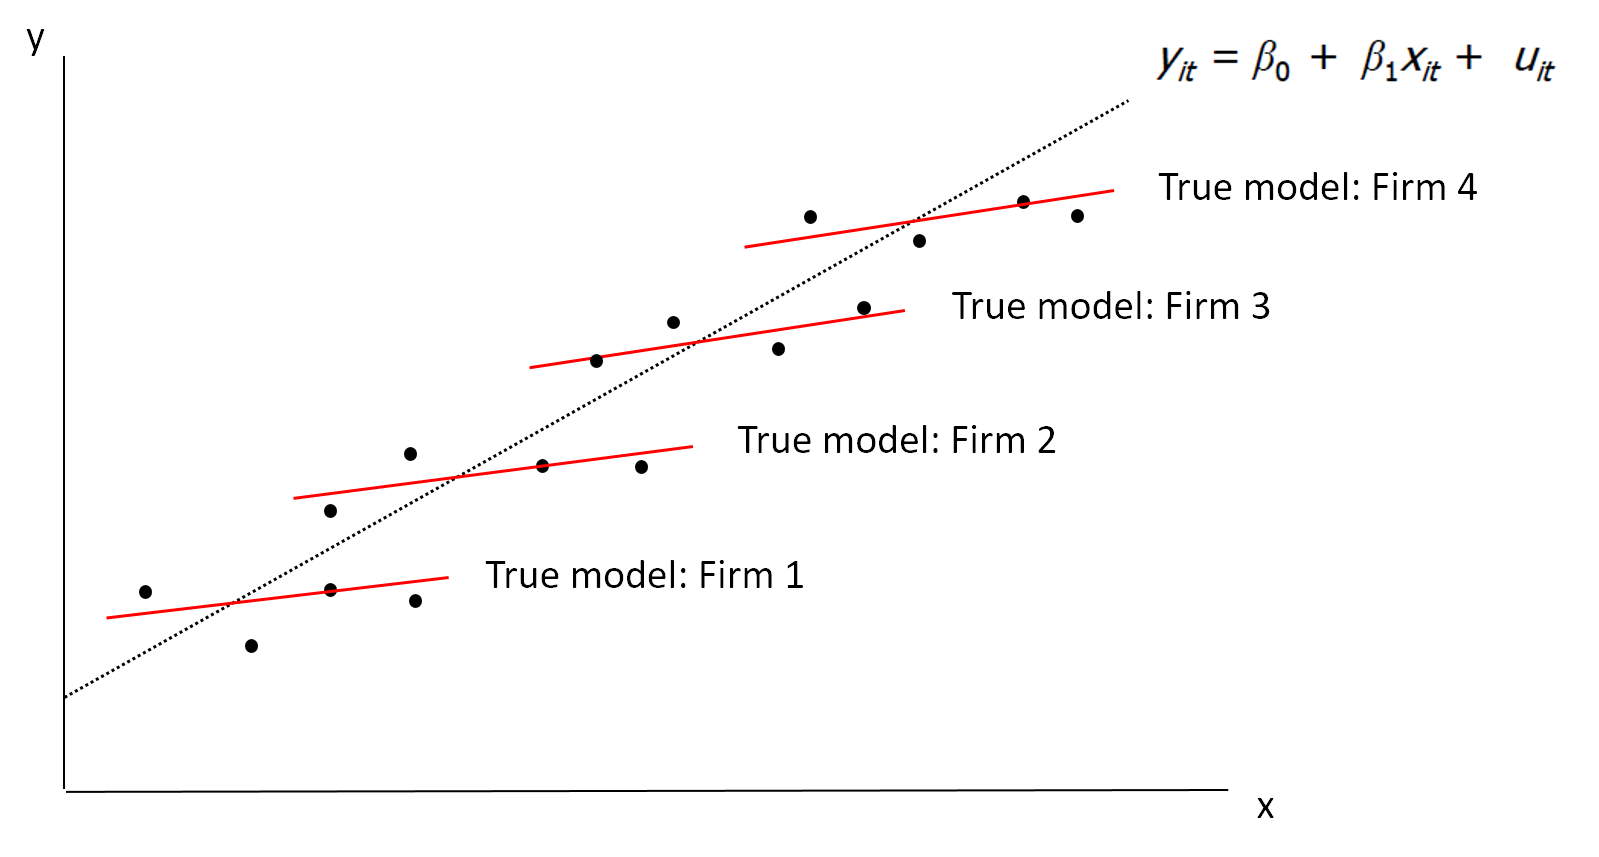
\includegraphics[width=\textwidth]{./img/Obrazek4}
\end{frame}
%---------------------------------
\begin{frame}{Basic features and motivation for panel data use}
\textbf{Variation for the dependent variable and regressors}
\begin{itemize}
\item Overall variation: variation over time and individuals.
\item Between variation: variation between individuals.
\item Within variation: variation within individuals (over time).
\end{itemize}
\tiny
\begin{table}[]
\centering
\label{Tab3}
\noindent\makebox[\textwidth]{%
\begin{tabular}{|c|c|c|c|c|c|c|c|c|}
\hline
Id  & Time & Variable & \begin{tabular}[c]{@{}c@{}}Individual\\ mean\end{tabular} & \begin{tabular}[c]{@{}c@{}}Overall\\ mean\end{tabular} & \begin{tabular}[c]{@{}c@{}}Overall\\ deviation\end{tabular} & \begin{tabular}[c]{@{}c@{}}Between\\ deviation\end{tabular} & \begin{tabular}[c]{@{}c@{}}Within\\ deviation\end{tabular} & \begin{tabular}[c]{@{}c@{}}Within\\ deviation\\ (modified)\end{tabular} \\ \hline
$i$ & $t$  & $x_{it}$ & $\overline{x}_i$ & $\overline{x}$ & $x_{it}-\overline{x}$ & $\overline{x}_{i}-\overline{x}$ & $x_{it}- \overline{x}_i$ & $x_{it}-\overline{x}_{i} + \overline{x}$ \\ \hline
1   & 1    & 9        & 10                                                        & 20                                                     & -11                                                         & -10                                                         & -1                                                         & 19                                                                      \\ \hline
1   & 2    & 10       & 10                                                        & 20                                                     & -10                                                         & -10                                                         & 0                                                          & 20                                                                      \\ \hline
1   & 3    & 11       & 10                                                        & 20                                                     & -9                                                          & -10                                                         & 1                                                          & 21                                                                      \\ \hline
2   & 1    & 20       & 20                                                        & 20                                                     & 0                                                           & 0                                                           & 0                                                          & 20                                                                      \\ \hline
2   & 2    & 20       & 20                                                        & 20                                                     & 0                                                           & 0                                                           & 0                                                          & 20                                                                      \\ \hline
2   & 3    & 20       & 20                                                        & 20                                                     & 0                                                           & 0                                                           & 0                                                          & 20                                                                      \\ \hline
3   & 1    & 25       & 30                                                        & 20                                                     & 5                                                           & 10                                                          & -5                                                         & 15                                                                      \\ \hline
3   & 2    & 30       & 30                                                        & 20                                                     & 10                                                          & 10                                                          & 0                                                          & 20                                                                      \\ \hline
3   & 3    & 35       & 30                                                        & 20                                                     & 15                                                          & 10                                                          & 5                                                          & 25                                                                      \\ \hline
\end{tabular}}
\end{table}
\end{frame}
%---------------------------------
\begin{frame}{Panel data models}
\underline{Panel data model -- a stylized and structured notation } \\
\medskip
$$y_{it} = \bm{g}_t \bm{\theta} + \bm{z}_i \bm{\delta} + \bm{w}_{it} \bm{\gamma} + a_i + u_{it}$$\\
\medskip
where \quad $i = 1,2, \dots, N$; $t = 1, 2, \dots, T$, \\
\medskip
$\bm{g}_t$ is a vector of aggregate time effects (often time dummies),\\
\medskip
$\bm{z}_i$ is a set of time-constant observed variables, \\
\medskip
$\bm{w}_{it}$ changes across $i$ and $t$ (for at least some units $i$ and time periods $t$), can include interactions among time-constant and time varying variables, \\
\medskip
$\bm{\theta, \delta}$ and $\bm{\gamma}$ -- regression coefficients 
\end{frame}
%---------------------------------
\begin{frame}{Panel data models}
\textbf{\underline{Panel data model - a structured notation example}} \\
\begin{align*}
\log(\textit{wage}_{it}) = \theta_0 & + \theta_1 d91_t + \theta_2 d92_t + \delta_1 \textit{female}_i + \delta_2 \textit{educ}_i +\\
& + \gamma_1 \textit{exper}_{it} + \gamma_2 (\textit{female} \times \textit{exper})_{it} + a_i + u_{it}
\end{align*}
Where $t = 1990, 1991, 1992$; \quad $i = 1, 2, \dots , \mytikzmark{100}{100}$. \\
For a balanced panel, $T \times N = 300$ \\
\vspace{0.2cm}
$d91_t$ and $d92_t$ are time dummies, \\
$\textit{female}_i$ and $\textit{educ}_i$ do not change over time \\(individuals in our dataset are not active students \dots ), \\
$\textit{exper}_{it}$ changes between individuals and across time periods,
$(\textit{female} \times \textit{exper})_{it}$ is an interaction element, changes between individuals and across time.
\begin{tikzpicture}[<-,overlay,remember picture,inner sep=1.5pt,shorten <=0.2em,font=\scriptsize]
\tikzset{
    mynode/.style={rectangle,draw=ProcessBlue,  fill=White, semithick, inner sep=.2em, minimum size=2em, text centered, text width=6em},
    myarrow/.style={->, >=stealth, thin, Red}
}
\node[mynode] at (4.9,3.44) (100*){We follow 100 individuals across three years.};
\draw[myarrow] (100*) -- ++   (100);
\end{tikzpicture}
\end{frame}
%---------------------------------
\section{Short panels -- estimation, inference \& testing}
\begin{frame}{Short panels -- estimation, inference \& testing}
    \begin{itemize}
        \item Estimation methods -- repetition from BSc courses
        \bigskip
        \item Choosing adequate estimators: assumptions and tests
        \bigskip
        \item Robust inference (autocorrelation and heteroscedasticity)
    \end{itemize}
\end{frame}
%---------------------------------
\subsection*{Estimation methods -- repetition from BSc courses}
\begin{frame}{LSDV regression}
In the model \quad  $y_{it} = \bm{x}_{it} \bm{\beta} + a_i + u_{it} \,$, \\
\bigskip
Elements $a_i$ are usually regarded as unobservable variables. \\
This approach gives appropriate interpretation of $\bm{\beta}$. \\
Traditional (old) approaches to fixed effects estimation view the $a_i$ as parameters to be estimated along with $\bm{\beta}$. \\
\bigskip
How to estimate $a_i$ values along with $\bm{\beta}$?\\
\medskip
\begin{itemize}
\item Define $N$ dummy variables - one for each cross-section. \\
(Amendment for dummy-variable trap is necessary.)
\smallskip
\item Convenient LSDV model expansion: use interactions to control for individual slopes for chosen regressors.
\end{itemize}
\end{frame}
%---------------------------------------------------------------------
\begin{frame}{FD estimator}
We can eliminate unobserved individual heterogeneity from the regression: \quad $y_{it} = \bm{x}_{it} \bm{\beta} + a_i + u_{it}$ \\ \smallskip
by first differences (FD) transformation: \\
$\Delta y_{it} = y_{it} - y_{i,t-1} = \Delta \bm{x}_{it} \bm{\beta} + \Delta a_i + \Delta u_{it} = \Delta \bm{x}_{it} \bm{\beta} + \Delta u_{it}$ \\ \medskip
\begin{itemize}
\item[$\checkmark$] Removes any unobserved heterogeneity.
\item[$\times$] We remove all time-invariant factors in $\bm{x}$.\\
If the time-invariant regressors are of no interest, this is \\a robust estimator.
\end{itemize} \medskip
Estimation can be done with FGLS (autocorrelation of transformed residuals), or OLS with HAC robust errors. \\
\medskip
FD is most suitable when we have $t = 1; 2$ – two period panel (FD may be used with more time periods, we have $N(T-1)$ observations after differencing)
\end{frame}
%---------------------------------------------------------------------
\begin{frame}{FD estimator – assumptions}
\begin{itemize}
\item[\textbf{FD.1}] Functional form: $y_{it} = \beta_1 x_{it1} + \dots + \beta_k x_{itk} + a_i + u_{it}$, $i = 1, \dots, N$, \ $t = 1, \dots, T$
\item[\textbf{FD.2}] We have random sample from cross-sectional units.
\item[\textbf{FD.3}] Each regressor changes in time at least for some $i$ and no perfect linear combination exists among regressors.
\item[\textbf{FD.4}] For each $i$ and $t$, \ $E (u_{it} \mid \bm{X}_i, a_i) = 0$. [Alt.: regressors are strictly exogenous conditional on unobserved effects: $\textnormal{corr}(x_{itj}, u_{is} \mid a_i)=0$, \quad $\forall \ t, s$]
\item[\textbf{FD.5}] Variance of differenced errors conditional on all regressors is constant: $\textnormal{var}(\Delta u_{it} \mid \bm{X}_i) = \sigma^2$, \quad $t= 2,3, \dots, T$. [homoscedasticity]
\item[\textbf{FD.6}] No serial correlation exists among differenced errors. $\textit{cov}(\Delta u_{it}, \Delta u_{is} \mid \bm{X}_i) = 0$, \quad $t \neq s$
\item[\textbf{FD.7}] Differenced errors are normally distributed conditional on all regressors $\bm{X}_i$.
\end{itemize}
\end{frame}
%---------------------------------
\begin{frame}{FD estimator – assumptions}
Under  \textcolor{blue}{\textbf{FD.1 - FD.4}}\\
FD estimator is unbiased. \\
FD estimator is consistent for fixed $T$ as $N \rightarrow \infty$.\\
For unbiasedness, $E (\Delta u_{it} \mid \bm{X}_i) = 0$ (for $t = 2,3, \dots$) is sufficient (instead of FD.4)\\
\medskip
Under \textcolor{blue}{\textbf{FD.1 - FD.6}}\\
FD estimator is BLUE (conditional on explanatory variables).\\
Asymptotic inference for FD estimator holds ($t$ and $F$ statistics asymptotically follow corresponding distributions).\\
\medskip
Under  \textcolor{blue}{\textbf{FD.1 - FD.7}}\\
FD estimator is BLUE (conditional on explanatory variables).\\
FD estimators - i.e. pooled OLS on first differences - are normally distributed ($t$ and $F$ statistics have exact $t$ and $F$ distributions).
\end{frame}
%---------------------------------
\begin{frame}{FD estimator}
\underline{\textbf{Problems related to the FD estimator:}}\\ \medskip
\begin{itemize}
\item First-differenced estimates will be imprecise if explanatory variables vary only to a small extent over time (no estimate possible if regressors are time-invariant).
\item Potentially, there is insufficient (lower) variability in differenced variables.
\item Without strict exogeneity of regressors (e.g. in the case of a lagged dependent variable /say, $y_{i,t-1}$/ among regressors or with measurement errors), adding further periods does not reduce inconsistency.
\item FD estimator may be worse than pooled OLS if explanatory variables are subject to measurement errors (errors in variables - EIV).
\end{itemize}
\end{frame}
%---------------------------------------------------------------------
\begin{frame}{FE estimator}
``Fixed'' means correlation of $a_i$ and $\bm{x}_{it}$, not that $a_i$ is non-stochastic.\\ \medskip
We can rewrite $y_{it} = \bm{x}_{it} \bm{\beta} + a_i + u_{it}$ as follows:\\
$y_{it} = \beta_1 x_{it1} + \dots + \beta_k x_{itk} + a_i + u_{it},$$
\hfill $$i = 1, \dots, N$, \ $t = 1, \dots,T$ \\ 
Now, \underline{for each $i$}, we \underline{average} the above equation \underline{over time}:\\
\medskip
${\overline{y}_i = \beta_1 \overline{x}_{i1} + \dots + \beta_k \overline{x}_{ik} + \overline{a}_i + \overline{u}_i}$\\ ($N$ equations with individual averages)\\
\medskip
By subtracting individual averages from the original observations (time-demeaning), we get:\\ \medskip
$\Rightarrow \boxed{[y_{it} - \overline{y}_{i}]} = \beta_1 \boxed{[x_{it1}-\overline{x}_{i1}]}+\dots+\beta_k \boxed{[x_{itk}-\overline{x}_{ik}]}+\boxed{[u_{it}- \overline{u}_i]}$\\
\medskip
Alternative notation: $\ddot{y}_{it} = \bm{\ddot{x}}_{it} \bm{\beta} + \ddot{u}_{it}$; where $\ddot{y}_{it} = y_{it} - \overline{y}_{i}$, etc.\\
\medskip
FE estimator, denoted $\bm{\hat{\beta}}_{FE}$, is the pooled OLS estimator applied to time-demeaned data.
\end{frame}
%---------------------------------------------------------------------
\begin{frame}{FE estimator}
\textbf{FE estimator:} by time demeaning, we get rid of the $a_i$ element - as it does not vary over time 
\medskip
\begin{itemize}
\item $a_i = \overline{a}_i \ \rightarrow \ a_i - \overline{a}_i = 0$
\item Intercept and all time-invariant regressors are also eliminated using the FE (within) transformation.
\end{itemize}
\medskip
After FE estimation, $a_i$ elements may be estimated as follows:\\ \medskip
$\hat{a}_i =\overline{y}_i - \hat{\beta}_1 \overline{x}_{i1} - \dots - \hat{\beta}_k \overline{x}_{ik},$ \ $i = 1, \dots, N$ \\
\medskip
However, in most practical applications, $a_i$ values bear limited useful information.\\ \medskip
For each C-S observation $i$, we loose one d.f. in estimation ~ \dots for each $i$, the demeaned errors $\ddot{u}_{it}$ add up to zero when summed over time. Hence \ $df = N(T-1)-k$
\end{frame}
%---------------------------------------------------------------------
\begin{frame}{FE estimator – assumptions}
\begin{itemize}
\item[\textbf{FE.1}] Functional form: $y_{it} = \beta_1 x_{it1} + \dots + \beta_k x_{itk} + a_i + u_{it}$, $i = 1, \dots, N$, \ $t = 1, \dots, T$
\item[\textbf{FE.2}] We have random sample from cross-sectional units.
\item[\textbf{FE.3}] Each regressor changes in time at least for some $i$ and no perfect linear combination exists among regressors.
\item[\textbf{FE.4}] For each $i$ and $t$, \ $E (u_{it} \mid \bm{X}_i, a_i) = 0$. [Alt.: regressors are strictly exogenous conditional on unobserved effects: $\textnormal{corr}(x_{itj}, u_{is} \mid a_i)=0$, \quad $\forall \ t, s$]
\item[\textbf{FE.5}] Variance of errors conditional on all regressors is constant: $\textnormal{var}(u_{it} \mid \bm{X}_i, a_i) = \textnormal{var}(u_{it}) = \sigma^2_u$, \quad $t= 1,2, \dots, T$. [homoscedasticity]
\item[\textbf{FE.6}] No serial correlation exists among idiosyncratic errors. $\textnormal{cov}(u_{it}, u_{is} \mid \bm{X}_i, a_i) = 0$, \quad $t \neq s$
\item[\textbf{FE.7}] Errors are normally distributed conditional on all regressors $(\bm{X}_i, a_i)$.
\end{itemize}
\end{frame}
%---------------------------------
\begin{frame}{FE estimator – assumptions}
Under \textcolor{blue}{\textbf{FE.1 - FE.4}} (identical to  \textcolor{blue}{\textbf{FD.1 - FD.4}})\\
FE estimator is unbiased. \\
FE estimator is consistent for fixed $T$ as $N \rightarrow \infty$.\\
\vspace{0.5cm}
Under \textcolor{blue}{\textbf{FE.1 - FE.6}}\\
FE estimator is BLUE.\\
FD is unbiased\\ \dots  \textcolor{blue}{\textbf{FE.6}} makes FE better (less variance) than FD.\\
Asymptotically valid inference for FE estimator holds ($t$ and $F$).\\
\vspace{0.5cm}
Under  \textcolor{blue}{\textbf{FE.1 - FE.7}}\\
FE estimator is BLUE and $t$ and $F$ statistics have exact $t$ and $F$ distributions.\\
FE estimators - i.e. pooled OLS on time demeaned data - are normally distributed.
\end{frame}
%---------------------------------
\begin{frame}{RE estimator}
\small 
If $a_i$ are uncorrelated with $\bm{x}_{it}$, then it may be appropriate to model the individual constant terms as randomly distributed across cross-sectional units. RE models are appropriate if C-S units are from \textbf{a large sample} (good asymptotic properties).
\bigskip

\begin{itemize}
\item RE models reduce the number of parameters estimated.
\item RE estimator potentially inconsistent if assumptions not met.
\item $y_{it} = \bm{x}_{it} \bm{\beta} + a_i + u_{it}$\\ \medskip
If we can assume that $a_i$ is uncorrelated with each explanatory variable: $\textnormal{corr}(\bm{x}_{it}, a_i) = 0$; \ $t = 1,2, \dots, T$ \\then we may drop $a_i$ from the equation and $\beta_j$ estimates will remain unbiased.\\
\item By dropping $a_i$ from the regression, we effectively create a new error term: $v_{it} = a_i + u_{it}$\\
\medskip
\item As $a_i$ is time-invariant, the random element $v_{it}$ contains a lot of ``inertia'', i.e. autocorrelation (unless $a_i = 0$).
\end{itemize}
\end{frame}
%---------------------------------
\begin{frame}{RE estimator - FGLS}
\small 
$y_{it} = \beta_0 + \beta_1 x_{it1} + \dots + \beta_k x_{itk} + v_{it};$\\
\bigskip
The quasi-demeaning (quasi-differencing) parameter $\theta$ is used for the FGLS estimation:\\ \medskip
$\theta = 1 - \big[ \sigma^2_u / (\sigma^2_u + T \sigma^2_{a}) \big]^{1/2}$, \quad  $0 \le \theta \le 1$\\ \medskip
where $\textit{var}(a_i) = \sigma^2_{a}$; \quad $\textit{var}(u_i) = \sigma^2_u$\\
\begin{itemize}
\item \small For each dataset, consistent estimators of $\sigma^2_{a}$ and $\sigma^2_u$ are available.\\
\item \small Their estimation is based on pooled OLS or FE. \\ Also, we use the fact that $\sigma^2_v = \sigma^2_{a} + \sigma^2_u$
\end{itemize}
RE estimator is a pooled OLS used on the quasi-demeaned data:\\ \medskip
{\footnotesize $$\boxed{[y_{it} - \theta \overline{y}_i]} = \beta_1 \boxed{[x_{it1}- \theta \overline{x}_{i1}]}+\dots+\beta_k \boxed{[x_{itk}- \theta \overline{x}_{ik}]}+\boxed{[a_i - \theta \overline{a}_i + u_{it}-\theta \overline{u}_i]}$$} \\ \medskip
(transformed errors follow G-M assumptions -- not autocorrelated)
\end{frame}
%---------------------------------
\begin{frame}{RE estimator - FGLS}
\
{\footnotesize $$\boxed{[y_{it} - \theta \overline{y}_i]} = \beta_1 \boxed{[x_{it1}- \theta \overline{x}_{i1}]}+\dots+\beta_k \boxed{[x_{itk}- \theta \overline{x}_{ik}]}+\boxed{[a_i - \theta \overline{a}_i + u_{it}-\theta \overline{u}_i]}$$}\\
\bigskip
Interestingly, the FGLS equation is a general form that encompasses both FE and pooled OLS:
\bigskip
\begin{align*}
\hat{\theta} \rightarrow 1 \quad & \rightarrow \quad \textnormal{RE}  \rightarrow \ \textnormal{FE}\\
\hat{\theta} \rightarrow 0 \quad & \rightarrow \quad \textnormal{RE}  \rightarrow \ \textnormal{Pooled}
\end{align*}
\end{frame}
%---------------------------------
\begin{frame}{RE estimator – Assumptions}
\footnotesize
\begin{itemize}
\item[\textbf{FE.1}] Functional form: $y_{it} = \beta_1 x_{it1} + \dots + \beta_k x_{itk} + a_i + u_{it}$, $i = 1, \dots, N$, \ $t = 1, \dots, T$
\item[\textbf{FE.2}] We have random sample from cross-sectional units.
\item[\textbf{FE.4}] $\forall \ i, t$: \ $E (u_{it} \mid \bm{X}_i, a_i) = 0$. [Alt.: $\textnormal{corr}(x_{itj}, u_{is} \mid a_i)=0$, \ $\forall \ t, s$]
\item[\textbf{FE.5}] Variance of idiosyncratic errors conditional on all regressors is constant: $\textnormal{var}(u_{it} \mid \bm{X}_i, a_i) = \textnormal{var}(u_{it}) = \sigma^2_u$, \quad $t= 1,2, \dots, T$. [homoscedasticity]
\item[\textbf{FE.6}] No serial correlation exists among idiosyncratic errors. $\textnormal{cov}(u_{it}, u_{is} \mid \bm{X}_i, a_i) = 0$, \quad $t \neq s$
\item[\textcolor{black}{\textbf{FE.7}}] [small sample normality of $u_{it}$ has little importance for RE estimator]
\end{itemize}
	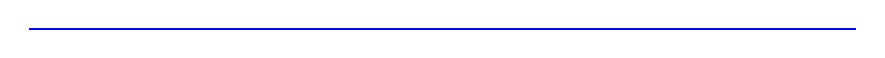
\begin{tikzpicture}
	\draw[thick, color=blue] (0,0) -- (10.5,0);
	\end{tikzpicture}
\begin{itemize}
\item[\textbf{RE.1}] There are no perfect linear relationships among explanatory variables. [replaces \textcolor{blue}{\textbf{FE.3}}]
\item[\textbf{RE.2}] In addition to \textcolor{blue}{\textbf{FE.4}}, the expected value of $a_i$ given all regressors is constant: $E(a_i \mid \bm{X}_i)=\beta_0$. [Rules out correlation between $a_i$ and $\bm{X}_i$]
\item[\textbf{RE.3}] In addition to \textcolor{blue}{\textbf{FE.5}}, variance of $a_i$ given all regressors is constant: $\textnormal{var}(a_i \mid \bm{X}_i)=\sigma^2_a$ [homoscedasticity imposed on $a_i$]
\end{itemize}
\end{frame}
%---------------------------------
\begin{frame}{RE estimator – Assumptions}
Under  \textcolor{blue}{\textbf{FE.1+FE.2+RE.1+(FE.4+RE.2)}}\\
RE estimator is consistent and asymptotically normal \\(for fixed $T$ as $N \rightarrow \infty$).\\
RE standard errors and statistics are not valid unless \textcolor{blue}{\textbf{(FE.5+RE.3)}} and  \textcolor{blue}{\textbf{FE.6}} conditions are met.\\
\bigskip
Under  \textcolor{blue}{\textbf{FE.1-FE.2+RE.1+(FE.4+RE.2)+(FE.5+RE.3)+FE.6}}\\
RE estimator is consistent and asymptotically normal \\(for fixed $T$ as $N \rightarrow \infty$).\\
RE standard errors and statistics are valid.\\
RE is asymptotically efficient 
\begin{itemize}
\item[-] lower st.errs. than pooled OLS
\item[-] for time-varying variables, RE estimator is more efficient than FE (FE cannot be used on time-invariant variables).
\end{itemize}
\end{frame}
%---------------------------------
\begin{frame}{CRE estimator}
Correlated Random Effects (CRE) estimator - a synthesis of the RE and FE approaches: 
\vspace{0.5cm}
\begin{itemize}
\item $a_i$ viewed as random, yet they can be correlated with $\bm{x}_{it}$.\\
\vspace{0.2cm}
Specifically, as $a_i$ do not vary over time, it makes sense to allow for their correlation with the time average of $x_{it}:\overline{x}_i = T^{-1} \sum^T_{t=1}x_{it}$
\vspace{0.2cm}
\item CRE allows for incorporation of time-invariant regressors (compare to FE).
\vspace{0.2cm}
\item CRE allows for convenient testing of FE vs. RE.
\end{itemize}
\end{frame}
%---------------------------------
\begin{frame}{CRE estimator}
CRE: The individual-specific effect $a_i$ is split up into a part that is related to the time-averages of the explanatory variables and a part $r_i$ (a time-constant unobservable) that is unrelated to the explanatory variables: 
\begin{align*}
\textnormal{For } y_{it} & =  \beta_1 x_{it} + a_i + u_{it}, \\
&\textnormal{~~we assume (a single-regressor illustration):}\\ 
a_i & = \alpha + \gamma \overline{x}_i + r_i \textnormal{,~~now: } \textnormal{corr}(r_i, \overline{x}_i) = 0 \Rightarrow \textnormal{corr}(r_i,x_{it}) = 0\\ 
&\textnormal{~~(because $\overline{x}_i$  is a linear function of  $x_{it}$)}
\end{align*}

By substituting for $a_i$ into the first equation, we obtain: \\
$y_{it} = \alpha + \beta_1 x_{it} + \gamma \overline{x}_i + r_i + u_{it}$ \\
\bigskip
\underline{This equation can be estimated using RE}\\
As $\gamma \overline{x}_i$ controls for the correlation between $a_i$ and $x_{it}$, \\$r_i$ is uncorrelated with regressors.
\end{frame}
%---------------------------------
\begin{frame}{CRE estimator}
CRE: \ $y_{it} = \alpha + \beta_1 x_{it} + \gamma \overline{x}_i + r_i + u_{it}$ \\
\medskip
\small CRE is a modified RE of the original equation $y_{it} =  \beta_1 x_{it} + a_i + u_{it}$: \\
\vspace{0.2cm}
with uncorrelated random effect $r_i$ but with the time averages as additional regressors. \\
\vspace{0.3cm}
\underline{The resulting CRE estimate for $\beta$ is identical to the FE estimator}. \\ \medskip
CRE allows for convenient testing of FE vs. RE:
	\begin{itemize}
	\item[$H_0$:] $\gamma = 0$ can be evaluated using $\hat{\gamma}_{\textit{CRE}}$ and appropriate (HCE) standard errors against
	\item[$H_1$:] $\gamma \neq 0$ [RE assumes $\gamma = 0$: reject $H_0\rightarrow$ reject RE in favor of FE]
	\end{itemize}

\begin{itemize}
    \item CRE is a versatile estimator. In terms of model specification, it allows for incorporation of time-invariant regressors into panel data models where $a_i$ is correlated with regressors.
\end{itemize}
\end{frame}
%---------------------------------
\begin{frame}{Arellano-Bond estimator (dynamic panels)}
Dynamic panel model example:\\
\medskip
$y_{it} = \delta_1 y_{i,t-1} + \bm{x}^{\prime}_{it} \bm{\beta} + a_i + u_{it}$\\
\medskip
\dots may be expanded using additional lags of the dependent variable or using lagged exogenous regressors.\\
\medskip
\small
\textbf{Nickel Bias}
\begin{itemize}
\item Related (mostly) to the lagged exogenous regressors $\bm{x}$
\item FEs take up some part of the dynamic effect and therefore dynamic panel data models lead to overestimated FEs and underestimated dynamic interactions. 
\item Whether the Nickel bias is significant in a particular model/dataset situation is an empirical question. Nevertheless, in theory this bias persists unless the number of time observations goes to infinity.
\item The inclusion of additional cross-sections to the dataset would worsen the bias in most cases.
\end{itemize}
\end{frame}
%---------------------------------
\begin{frame}{Arellano-Bond estimator (dynamic panels)}
\textbf{Arellano-Bond (AB) estimator} \\ \medskip
\begin{itemize}
\item The model is transformed into first differences to eliminate the individual effects:\\
$\Delta y_{it} = \delta_1 \Delta y_{i,t-1} + \Delta \bm{x}^{\prime}_{it} \bm{\beta} + \Delta u_{it}$, 
\medskip
\item then a generalized method of moments (GMM) approach is used to produce asymptotically efficient estimates of the coefficients.
\medskip
\item AB is based on IVR (we need instruments for lagged dependent variable as this is an endogenous regressor in the FD-transformed model ($\Delta y_{i,t-1}$ correlated to $\Delta u_{it}$).
\medskip
\item \textcolor{red}{Warning:} AR(2) / not AR(1) / autocorrelation in residuals of the AB-estimated model renders the AB estimator inconsistent. After using the AB estimator, always test for AR(2) autocorrelation in the residuals!
\end{itemize}
\end{frame}
%---------------------------------
\subsection*{Choosing adequate estimators -- assumptions and tests}
\begin{frame}{Choosing adequate estimators -- assumptions and tests}
\begin{itemize}
    \item Poolability tests (pooled regression vs other estimators)
    \medskip
    \item Cross sectional dependency
    \medskip
    \item Estimator selection (FD vs FE;  FE vs RE)
    \medskip 
    \item Autocorrelation, heteroscedasticity, and robust inference
\end{itemize}
\end{frame}
%--------------------------------- 
\begin{frame}{Choosing adequate estimators -- assumptions and tests}
We start by generalization of the (short) panel data model:
\begin{itemize}
   \medskip
    \item[a)] Model with individual effects: 
    $$y_{it} = \alpha + \beta_{1} x_{it1} + \dots + \beta_K x_{itK} + a_i + \nu_{it}$$
    \item[b)] Model with time effects: 
    $$y_{it} = \alpha + \beta_{1} x_{it1} + \dots + \beta_K x_{itK} + \lambda_t + \nu_{it}$$  
    \item[c)] Model with twoways effects: 
    $$~~~~~y_{it} = \alpha + \beta_{1} x_{it1} + \dots + \beta_K x_{itK} + a_i + \lambda_t + \nu_{it}$$\\ \medskip
    \item For short panels, we often apply models with individual effects only -- and use time dummies if necessary.
    \item \textbf{Some} of the following test are designed for different variants of unobserved effects.
    \item In principle, unobserved time effects are dealt with the same way as unobserved individual effects.
\end{itemize}
\end{frame}
%--------------------------------- 
\begin{frame}{LSDV-based test for individual intercepts}
\small
\begin{itemize}
    \item Null hypothesis of common  intercept ($H_0:~a_1 = a_2 = \cdots = a_N$) is tested against the alternative of individual-specific intercepts. Common slopes (the same $\beta$-coefficients across CS units) are assumed (not tested).
    \medskip
    \item Test designed for individual effects (other variants by analogy).
    \medskip
    \item Unrestricted model: $y_{it} = \alpha + \bm{d}^{\prime}\bm{\delta} + \bm{x}_t^{\prime} \bm{\beta} + u_{it}$ \\ \medskip
    where $\bm{d}$ is a vector of CSID-based dummy variables and $\bm{\delta}$ is a vector of regression coefficients ($N-1$ dummies used to avoid dummy variable trap).
    \medskip
    \item Restricted model: $~~y_{it} = \alpha + \bm{x}_t^{\prime} \bm{\beta} + u_{it}$.
    \medskip
    \item Can be implemented as an $F$-test for linear (zero) restrictions: \\Pooled regression is compared to LSDV model.
\end{itemize}
\end{frame}
%--------------------------------- 
\begin{frame}{\texttt{pooltest()} -- \textit{F}-test of stability (Chow test)}
\small 
\begin{itemize}
    
    \smallskip
    \item Allows for different intercepts \& tests for equal slopes \\in all CS-units. \texttt{R} implementation compares pooling and FE estimators. Algorithm outline:
    \begin{itemize}
        \item[1] Estimate model separately for each CS unit (ignore $a_i$).
        \item[2] Compare with FE estimator (individual intercept, common slopes on regressors) using an $F$-test 
        \item Are the slopes ($\beta$-coefficients) identical among CS-units?
    \end{itemize}
    \smallskip
    \item \textbf{Drawback:} test cannot handle time-invariant regressors -- as the unrestricted model is estimated individually for each CS-unit, such regressors are perfectly correlated with the intercept. With FE estimator, all time-invariant regressors are eliminated. 
    \medskip
    \item Single-regressor example:\\ \medskip Unrestricted model: $y_{it} = \alpha + \beta_{i1} x_{it} + a_i + u_{it}, \quad i=1,2,\dots,N$\\ \smallskip Restricted model: $\,~~y_{it} = \alpha + \beta_1 x_{it} + a_i + u_{it},$
\begin{itemize}
    \item[] $H_0:~\beta_{11}=\beta_{21}=\dots=\beta_{N1}$  
    \item[] $H_1:~\neg H_0$
\end{itemize}
\end{itemize}
\end{frame}
%---------------------------------------------------------------------
\begin{frame}{\texttt{pooltest()} -- \textit{F}-test of stability (Chow test)}
\vspace{2.5cm}
\vfill
\bigskip
$\qquad F=\frac{ \mytikzmark{SSRr}{\textit{SSR}_r}- \mytikzmark{SSRur}{\textit{SSR}_{ur}}}{\textit{SSR}_{ur}} \cdot \frac{(NT-N-NK)}{(N-1)K};$ \\
\bigskip
{\small under $H_0$ of common slopes (no structural break),\\ \medskip $\qquad F \sim F[(N-1)K, (NT- \mytikzmark{TTk}{\circledd{$N-NK$)}}]$} \\
\bigskip
\begin{itemize}
\item \texttt{R} implementation: \texttt{pooltest()} from the \texttt{\{plm\}} package.
\end{itemize}
\begin{tikzpicture}[<-,overlay,remember picture,inner sep=1.5pt,shorten <=0.2em,font=\scriptsize]
\tikzset{
    mynode/.style={rectangle,draw=blue, dashed, fill=white, semithick, inner sep=.2em, minimum size=2em, text centered, text width=9em},
    myarrow/.style={->, >=stealth, thin, blue}
}
\node[mynode] at (1.8,7.2) (SSRr*){$\textit{SSR}_r$: restricted model – allow for different $a_i$, impute common slopes.};
\draw[myarrow] (SSRr*) -- ++   (SSRr);
	\node[mynode] at (5.5,7.2) (SSRur*){$\textit{SSR}_{ur}$:run a regression for each of the CS units. $\textit{SSR}_{ur} = 			\textit{SSR}_1 + \textit{SSR}_2 + \dots + \textit{SSR}_N$};
	\draw[myarrow] (SSRur*) -- ++   (SSRur);
		\node[mynode] at (9.3,7.2) (TTk*){$N + NK$ parameters estimated in the unrestricted model, $K$ is \# regressors};
		\draw[myarrow] (TTk*) -- ++   (TTk);
\end{tikzpicture}
\end{frame}
%---------------------------------------------------------------------
\begin{frame}{\texttt{pFtest()} for unobserved effects}
\small 
$y_{it} = \alpha + \bm{x}^{\prime}_{it} \bm{\beta} + a_i + \lambda_t + \nu_{it}$\\ \medskip
\begin{itemize}
    \item Generalization of the previous test. \\ \medskip $F$-test of unobserved effects based on the comparison of ``pooling'' and ``within'' models. Significances of either ``individual'', ``time'' or ``twoways'' effects can be tested.
    \medskip
    \item  Based on comparing FE-estimator against the pooling model. 
    \medskip 
    \item d.f. of the $F$-test statistic depend on the number of observations and parameters restricted:\\
    \texttt{df1} is the number of restrictions (parameters restricted), \\
    \texttt{df2} $= N(T-1)~-$ (\# parameters in the unrestricted model)
    \medskip
    \item Hence, two main arguments to the test function are \texttt{plm}-estimated ``pooling'' and ``within'' models. 
    \medskip
    \item Implementation: \texttt{pFtest()} from the \texttt{\{plm\}} package
\end{itemize}    
\end{frame}
%---------------------------------------------------------------------
\begin{frame}{Honda (1985) test for individual and time effects}
\begin{itemize}
    \item Using OLS-based (``pooling'') residuals, we test the null hypothesis of redundant individual $(a_i)$ and/or time $ (\lambda_t) $ effects.
    \bigskip
    \item This LM-based tests uses residuals of the pooling model. \\In \texttt{R}, if performed on RE of FE model, corresponding pooling model is calculated internally first. 
    \bigskip
    \item Implementation: \\ \medskip \texttt{plmtest(..., type="honda")} from the \texttt{\{plm\}} package
\end{itemize}
\end{frame}
%---------------------------------------------------------------------
\begin{frame}{Honda (1985) test for individual and time effects}
Panel model cast as: \\ \bigskip
\begin{itemize}
    \item $y_{it} = \alpha + \bm{x}^{\prime}_{it} \bm{\beta} + u_{it} \qquad$    where $u_{it}=a_i + \lambda_t + \nu_{it}$
    \bigskip
    \item Assumptions for Honda (1985) test: \\ \medskip {\it i.i.d.} individual effects: $a_i \sim N(0,\sigma^2_{a})$; \\{\it i.i.d.} time effects: $\lambda_t \sim N(0,\sigma^2_{\lambda})$; \\{\it i.i.d.} idiosyncratic errors: $\nu_{it} \sim N(0,\sigma^2_{\nu})$.
    \bigskip
    \item Null hypotheses to be tested:
    \medskip
    \begin{itemize}
        \item $H_0^{a}: \sigma^2_{a} = 0 \qquad \qquad$ ~~~(no individual effects)
        \smallskip
        \item $H_0^{\lambda}: \sigma^2_{\lambda} = 0 \qquad \qquad$ ~~~(no time effects)
        \smallskip
        \item $H_0^{a \lambda}: \sigma^2_{a} = \sigma^2_{\lambda} = 0 \qquad \,$ (no individual nor time effects)
    \end{itemize}
\end{itemize}
\end{frame}
%---------------------------------------------------------------------
\begin{frame}{Honda (1985) test for individual and time effects}
\small
$y_{it} = \alpha + \bm{x}^{\prime}_{it} \bm{\beta} + u_{it} \qquad$    where $u_{it}=a_i + \lambda_t + \nu_{it}$\\ \medskip Balanced panel assumed. \bigskip
\begin{itemize}
    \item Error component in matrix form: \\ \smallskip
    $\bm{u}_i = \left( u_{i1}, u_{i2}, \dots, u_{iT} \right)^{\prime}$ and $\bm{u} = \left( \bm{u}_1^{\prime}, \bm{u}_2^{\prime}, \dots, \bm{u}_N^{\prime} \right)^{\prime}$ \\ \smallskip
    $\bm{u}_i$ is $T \times 1$ and $\bm{u}$ is $NT \times 1$.
    \medskip
    \item In matrix form, $\bm{u}$ can be cast as: \\
    $\bm{u} = \bm{D}_{a} \bm{a} + \bm{D}_{\lambda} \bm{\lambda} + \bm{\nu}$ \\ \smallskip
    where \\$\bm{a} = (a_1, \dots, a_N)^{\prime}$, \\$\bm{\lambda} = (\lambda_1, \dots, \lambda_T)^{\prime}$, \\$\bm{\nu}$ follows the structure of $\bm{u}$,\\
    $\bm{D}_{a} = (\bm{I}_N \otimes \bm{\iota}_T)$ i.e. $\bm{I}_N$ with each row repeated $T$-times; $(NT \times N)$, \\
    $\bm{D}_{\lambda} = ( \bm{\iota}_N \otimes \bm{I}_T )$ i.e. $\bm{I}_T$ stacked vertically $N$-times; $(NT \times T)$, \\ 
    note that time is the ``fast index'' here.
    \end{itemize}
\end{frame}
%---------------------------------------------------------------------
\begin{frame}{Honda (1985) test for individual and time effects}
$y_{it} = \alpha + \bm{x}^{\prime}_{it} \bm{\beta} + u_{it} \qquad$    where $u_{it}=a_i + \lambda_t + \nu_{it}$\\ \medskip

$\bm{u} = \bm{D}_{a} \bm{a} + \bm{D}_{\lambda} \bm{\lambda} + \bm{\nu}$ \\ \vspace{0.3cm} \hrule \bigskip
\begin{itemize}
    \item $\bm{D}_{a} \bm{D}_{a}^{\prime} = \left(\bm{I}_N \otimes \bm{J}_T \right)$ i.e. block-diagonal matrix of $\bm{J}_T$-matrices \\where $\bm{J}_T=\iota_T \iota_T^{\prime}$  ($\bm{J}_T$ is a $T \times T$ matrix of ones).
    \medskip
    \item $\bm{D}_{\lambda} \bm{D}_{\lambda}^{\prime} = \left(\bm{J}_N \otimes \bm{I}_T   \right)$ i.e. $N\times N$ array of $\bm{I}_T$-matrices.
    \medskip
    \item Now, we define\\ \medskip
    $A_r = \left[ \left( \frac{\bm{u}^{\prime}\bm{D}_r \bm{D}_r^{\prime} \bm{u}}{\bm{u}^{\prime}\bm{u}} \right) - 1 \right]$ for $r=a$ or $r=\lambda$.
    \end{itemize}
\end{frame}
%---------------------------------------------------------------------
\begin{frame}{Honda (1985) test for individual and time effects}
$y_{it} = \alpha + \bm{x}^{\prime}_{it} \bm{\beta} + u_{it} \qquad$    where $u_{it}=a_i + \lambda_t + \nu_{it} \qquad$ \\Balanced panel assumed.\\ \vspace{0.3cm} \hrule \medskip
\begin{itemize}
    \item Honda (1985) provides (uniformly most powerful) {\it LM} statistics for $H_0^{a}: \sigma_{a}^2=0$ against a one-sided $H_1^{a}: \sigma_{a}^2>0$:
    $$
    \textnormal{HO}_{a} = \sqrt{\frac{NT}{2(T-1)}} ~ A_{a} ~ \underset{H_0}{\rightarrow}~N(0,1)
    $$ \\ \medskip
    \item Similarly, for $H_0^{\lambda}: \sigma_{\lambda}^2=0$ against a one-sided $H_1^{\lambda}: \sigma_{\lambda}^2>0$:
    $$
    \textnormal{HO}_{\lambda} = \sqrt{\frac{NT}{2(T-1)}} ~ A_{\lambda} ~ \underset{H_0}{\rightarrow}~N(0,1)
    $$
\end{itemize}    
\end{frame}
%---------------------------------------------------------------------
\begin{frame}{Honda (1985) test for individual and time effects}
$y_{it} = \alpha + \bm{x}^{\prime}_{it} \bm{\beta} + u_{it} \qquad$    where $u_{it}=a_i + \lambda_t + \nu_{it} \qquad$ \\Balanced panel assumed.\\ \vspace{0.3cm} \hrule \medskip
\begin{itemize}
    \item Honda (1985) provides a test statistic for\\ \vspace{0.3cm} $H_0^{a \lambda}: \sigma_{a}^2=\sigma_{\lambda}^2=0$ against a one-sided alternative
    \\(not derived as a uniformly most powerful {\it LM} statistics):\\ \medskip
    $$
    \textnormal{HO}_{a \lambda} = \frac{\textnormal{HO}_{a}+\textnormal{HO}_{\lambda}}{\sqrt{2}} {\rightarrow}~N(0,1)
    $$
    \medskip
    \item Honda (1985) statistics can be generalized to the unbalanced case -- see e.g.: \footnotesize{\textcolor{blue}{\underline{http://www.eviews.com/help/}}}
\end{itemize}    
\end{frame}
%---------------------------------------------------------------------
\subsection*{Cross sectional dependency}
\begin{frame}{Cross-sectional dependency (XSD)}
\begin{itemize}
    \item In principle, similar to serial correlation in TS data.
    \medskip
    \item Can arise if individuals respond to common shocks or if spatial autocorrelation processes are present, relating individuals based on their distances (spatial models).
    \medskip
    \item If XSD is present, the consequence is, at a minimum, inefficiency of the usual estimators and invalid inference when using the standard covariance matrix.
    \medskip
    \item In \texttt{\{plm\}}, only misspeciffication tests to detect XSD are available – no robust method to perform valid inference in its presence.
    \medskip
    \item In case of spatially determined XSD, spatial panel econometric models should be used (discussed separately).
\end{itemize}
\end{frame}
%---------------------------------
\begin{frame}{Cross-sectional dependency (XSD)}
\small
\begin{figure}[htbp] 
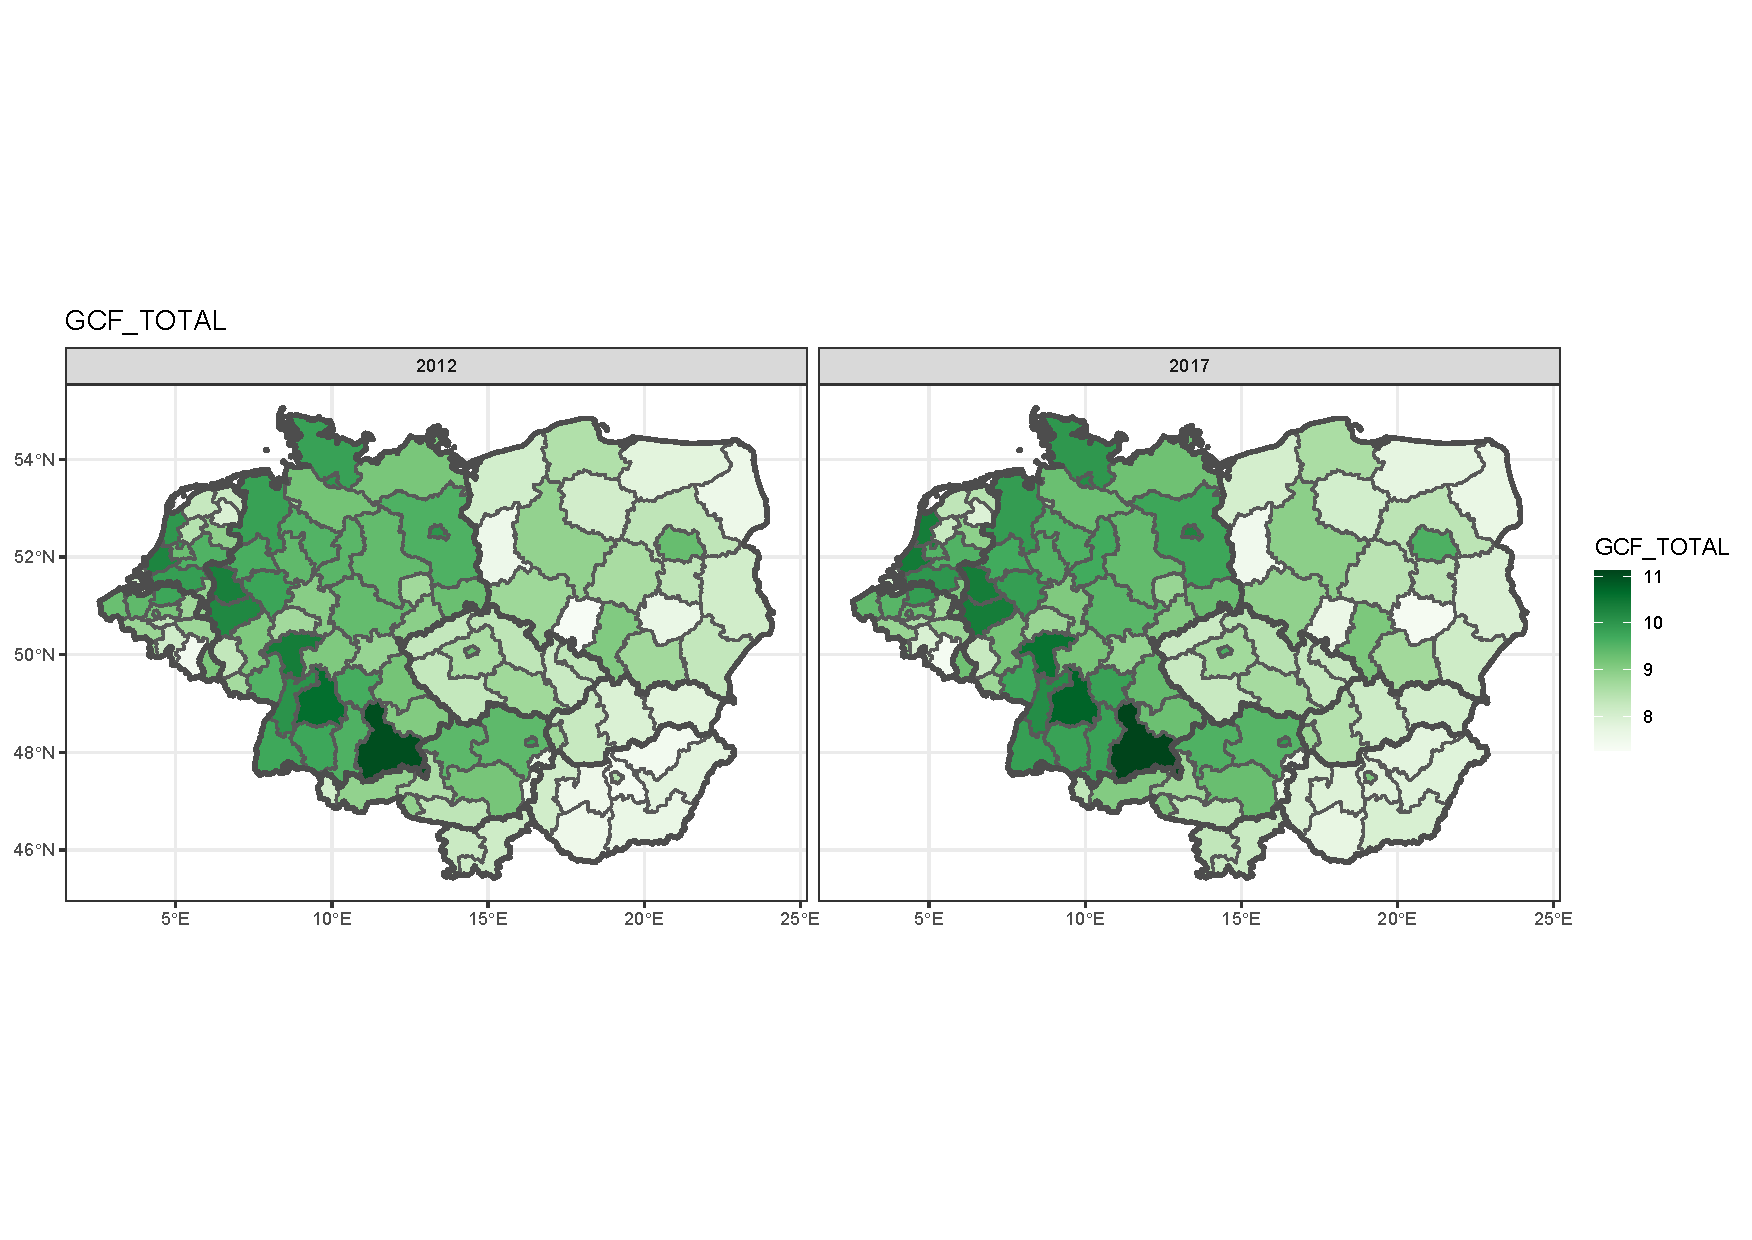
\includegraphics[trim = 0cm 5cm 0cm 5.7cm, clip, width=1\textwidth]{img/GCF_total.pdf}
\caption{\small{Total gross fixed capital formation; 2015 fixed prices, log-transformed EUR values, years 2012 and 2017 shown}} \label{fig:choropleth2}
\end{figure}
\begin{itemize}
    \item Spatial dependency is a common form of XSD. For details, see:\\
    \textsubscript{ \textcolor{Blue}{\url{https://cran.r-project.org/web/packages/spatialreg/index.html}} }
    \medskip
    \item Other forms of XSD may be linked to non-spatially defined groups (e.g. on social networks), etc.
\end{itemize}
\end{frame}
%---------------------------------
\begin{frame}{Cross-sectional dependency (XSD) test}
\small
\begin{itemize}
    \item \texttt{pcdtest()} from the \texttt{\{plm\}} package:
    \medskip
    \item Test based on transformations of the correlation coefficient of model residuals, defined as
    $$
    \hat{\rho}_{ij}=\frac{\sum_{t=1}^T \hat{u}_{it}\hat{u}_{jt}}
    {\left(\sum_{t=1}^T \hat{u}_{it}^2 \right)^{1/2} \left(\sum_{t=1}^T \hat{u}_{jt}^2 \right)^{1/2} }
    $$
    i.e. -- we use averages over the time dimension of pairwise correlation coefficients for each pair of CS-units.
    \bigskip
    \item Pesaran's CD test (Pesaran, 2004):
    $$
    \textnormal{CD} = \sqrt{\frac{2}{N(N-1)}}
    \left( \sum_{i=1}^{N-1} \sum_{j=i+1}^N \sqrt{T_{ij}}\, \hat{\rho}_{ij}
    \right)  \underset{H_0}{\rightarrow} N(0,1)
    $$
    CD test is appropriate in both $N$ and $T$-asymptotic settings. \\Also, CD test has good performance in samples of any practically relevant size and is robust to a variety of settings.
\end{itemize}
\end{frame}
%---------------------------------
\subsection*{Estimator selection (FD vs FE; FE vs RE)}
\begin{frame}{Estimator selection (FD vs FE; FE vs RE)}
\begin{itemize}
    \item FD vs FE estimators
    \bigskip
    \item FE vs RE estimators
\end{itemize}    
\end{frame}
%---------------------------------
\begin{frame}{FE vs FD estimator}
\begin{itemize}
\item For $T=2$, FE and FD estimators produce identical estimates and inference. (FE must include a time dummy for the second period to be actually identical to the FD estimation output)
\medskip
\item For $T>2$, FE and FD are both unbiased under \\FE.1 - FE.4. Both FE and FD are consistent for fixed $T$ as $N \rightarrow \infty$
\medskip
\item If $u_{it}$ is not serially correlated, FE is more efficient than FD
\medskip
\item If $u_{it}$ follows a random walk (hence $\Delta u_{it}$ is serially uncorrelated) FD is better than FE.
\medskip
\item If $u_{it}$ shows some level of positive serial correlation (not a random walk), FD and FE may not be easily compared. For negative correlation of $u_{it}$, we prefer FE.
\end{itemize}
\end{frame}
%---------------------------------
\begin{frame}{FE vs FD estimator}
\begin{itemize}
\item As the time dimension increases, especially if non-stationary series are involved, FE may lead to spurious regression problems, while the FD help us transforming integrated series into weakly dependent series.
\medskip
\item If strict exogeneity is violated, both FE and FD are biased. However, FE is likely to have less bias than FD (unless $T=2$). The bias of FD does not depend on $T$, while the bias in FE tends to zero at rate $1/T$.
\medskip
\item \dots it may be a good idea to use both FD and FE. If the results are not method-sensitive, so much the better. If the results from FE and FD differ significantly, we sometimes report both.
\end{itemize}
\end{frame}
%---------------------------------
\begin{frame}{FD vs FE estimator: Wooldridge's FD-based test}
\small
$y_{it} = \alpha + \bm{x}^{\prime}_{it} \bm{\beta} + a_i + \nu_{it}$\\ \medskip
\begin{itemize}
    \item Serial correlation test that can be used as a specification test to choose the most efficient estimator -- FD vs FE.
    \item If $\nu_{it}$ are not serially correlated, then: 
    \begin{itemize}
          \item[a)] FE is more efficient than FD.
          \item[b)] Residuals in the FD model: $e_{it} = \nu_{it}-\nu_{i,t-1}$ are correlated, \\with~ $\textnormal{cor}\left(e_{it},e_{i,t-1}\right)=-0.5$.
        \end{itemize}
        \item For models with individual effects, the test can be based on estimating the model $\hat{e}_{it}=\delta \hat{e}_{i,t-1}+\eta_{it}$ based on residuals of the FD model, where we test $H_0: \delta=-0.5$, corresponding to the null of no serial correlation in the original (undifferenced) residuals $\nu_{it}$. 
        \medskip
        \item If this $H_0$ is not rejected, we would prefer FE.
        \medskip
        \item Implementation: \texttt{pwfdtest()} from the \texttt{\{plm\}} package. \\ \smallskip  Test does not rely on large–T asymptotics and has good properties in short panels.
\end{itemize}
\end{frame}
%---------------------------------
\begin{frame}{FD vs FE estimator: Wooldridge's FD-based test}
$y_{it} = \alpha + \bm{x}^{\prime}_{it} \bm{\beta} + a_i + \nu_{it}$\\ \medskip
\begin{itemize}
    \item If $\nu_{it}$ follow a random walk: 
    \begin{itemize}
          \item FD is more efficient than FE.
          \item Residuals in the FE model: $\nu_{it}=\nu_{i,t-1}+e_{it}$.
          \item Residuals in the FD model: $e_{it} = \nu_{it}-\nu_{i,t-1}$ are not serially correlated, \\(definition of a random walk for $\nu_{it}$).
        \end{itemize}
        \smallskip
        \item \texttt{pwfdtest(..., h0="fd")} \\
        $H_0:$ no serial correlation in FD-errors $e_{it}$, \\if not rejected, use FD.
        \smallskip
        \item \texttt{pwfdtest(..., h0="fe")} \\
        $H_0:$ no serial correlation in FE-errors $\nu_{it}$, \\if not rejected, use FE.
        \smallskip
        \item If both rejected, whichever estimator is chosen will have serially correlated errors: use the autocorrelation-robust covariance estimators.
    \smallskip
\end{itemize}
\end{frame}
%---------------------------------
\begin{frame}{RE vs FE estimator: Hausman test}
\small
\begin{itemize}

    \item \textbf{Hausman test} is based on the comparison of two sets of estimates -- RE and FE.
    \bigskip
    \item A classical application of the Hausman test for panel data is to compare the coefficient vectors and corresponding covariance matrices of FE and RE estimators:
    $$H=(\hat{\bm{\beta}}_{FE} - \hat{\bm{\beta}}_{RE})^T [\widehat{\textnormal{Avar}}(\hat{\bm{\beta}}_{FE}) - \widehat{\textnormal{Avar}}(\hat{\bm{\beta}}_{RE})]^{-1} (\hat{\bm{\beta}}_{FE} - \hat{\bm{\beta}}_{RE}) \underset{H_0}{\sim} \chi^2(m)$$
    where $m$ is the number of regressors varying across $i$ and $t$.
    \smallskip
    \begin{itemize}
    \item[$H_0$] $\textnormal{cov}(\bm{x}_{it},a_i) = 0$ \dots i.e. the crucial RE assumption holds, both FE and RE are consistent (RE is efficient). \\ \smallskip
    \item[$H_1$] RE assumptions violated.
    \end{itemize}
    \medskip
    \item Implementation: \texttt{phtest()} from the \texttt{\{plm\}} package

\end{itemize}
\end{frame}
%---------------------------------
\begin{frame}{RE vs FE estimator: Hausman test}

\small $$H=(\hat{\bm{\beta}}_{FE} - \hat{\bm{\beta}}_{RE})^T [\widehat{\textnormal{Avar}}(\hat{\bm{\beta}}_{FE}) - \widehat{\textnormal{Avar}}(\hat{\bm{\beta}}_{RE})]^{-1} (\hat{\bm{\beta}}_{FE} - \hat{\bm{\beta}}_{RE}) \underset{H_0}{\sim} \chi^2(m)$$
\begin{itemize}
    \item If $\hat{\bm{\beta}}_{FE}$ and $\hat{\bm{\beta}}_{RE}$ do not differ too much [or when the asymptotic variances are relatively large] we do not reject $H_0$. 
    \medskip
    \item If we may assume RE assumptions hold, both RE and FE are consistent, RE is efficient. 
    \medskip
    \item For asymptotic variance estimators ($\widehat{\textnormal{Avar}}$), see Wooldridge (2010). 
    \medskip
    \item If we reject $H_0$, we need to assume that RE assumptions are violated $\rightarrow$ RE is not consistent [we use FE].
\end{itemize}
\end{frame}
%---------------------------------
\begin{frame}{RE vs FE estimator: CRE-based test}
$$ \textnormal{CRE:}~~y_{it} = \alpha + \beta_1 x_{it} + \gamma \overline{x}_i + r_i + u_{it}$$ \\ \bigskip

CRE allows for FE vs. RE testing: \\ \medskip
	\begin{itemize}
	\item[$H_0$:] $\gamma = 0$, i.e. RE assumptions hold -- can be evaluated using $\hat{\gamma}_{\textit{CRE}}$ and appropriate (HCE) standard errors.
	\medskip
	\item[$H_1$:] $\gamma \neq 0$ [reject $H_0\rightarrow$ reject RE in favor of FE]
	\end{itemize}
\end{frame}
%---------------------------------
\subsection*{Autocorrelation, heteroscedasticity, and robust inference}
\begin{frame}{Autocorrelation, heteroscedasticity, and robust inference}
\begin{itemize}
    \item Autocorrelation \& heteroscedasticity in short panels
    \medskip
    \item Autocorrelation \& heteroscedasticity tests
    \medskip
    \item Robust inference
\end{itemize}
\end{frame}
%--------------------------------- 
\begin{frame}{Autocorrelation \& heteroscedasticity in short panels}
$$y_{it} = \bm{x}_{it} \bm{\beta} + a_i + u_{it}$$

\begin{itemize}
\small
    \item \underline{Serial correlation (between-period correlation)} \\
    $u_{it} = \Bigg\{ \parbox{5cm}{$\boxed{\rho \ } u_{i,t - 1} + \varepsilon_{it} \\ \boxed{\rho_i} u_{i,t - 1} + \varepsilon_{it} $}$
    \medskip
    \item \underline{Correlation between cross-sectional units (XSD)}\\
    $H_0$ of no C-S dependence may be written as follows:\\ \smallskip
    $\rho_{ij} = \textit{corr}(u_{it}, u_{jt}) = 0 \textit{ \ for \ } i \neq j$ \\ \smallskip
    (XSD discussed separately, worth mentioning here \\as it is a type of autocorrelation).
    \medskip
    \item \underline{Heteroscedasticity} (RE-model example):\\
    $\textit{var}(v_{it} \mid \bm{X}_i) = \sigma^2_{a_i} + \textit{var}(u_{it} \mid \bm{X}_i) = \Bigg\{ \parbox{2cm}{$\sigma^2_{a_i} + \boxed{\sigma^2_{u_i}} \\ \sigma^2_{a_i} + \boxed{\sigma^2_{u_{t}} }$}$\\ ~\\ \medskip
\end{itemize}
\end{frame}
%---------------------------------
\begin{frame}{Serial correlation tests (RE model)}
\small 
\vspace{-0.2cm}
\begin{itemize}
    \item \texttt{pwtest()} ~~ Unobserved effects: ``Wooldridge''-type test
    \smallskip 
    \item $W = \frac{\displaystyle\sum_{i=1}^N 
        \displaystyle\sum_{t=1}^{T-1}
        \displaystyle\sum_{s=t+1}^T \hat{u}_{it}\hat{u}_{is}}
        {\left[\displaystyle\sum_{i=1}^N \left(
        \displaystyle\sum_{t=1}^{T-1}
        \displaystyle\sum_{s=t+1}^T \hat{u}_{it}\hat{u}_{is}
        \right)^{\!2}~ \right]^{1/2}}~
        \underset{H_0}{\sim}~ N(0,1)$;~~(asympt.), \\test does not rely on homoscedasticity assumptions.
    \medskip
    \item $H_0: \sigma_{a}^2 = 0$, i.e., that there are no unobserved effects in the residuals (of RE model).
    \item Test has power both against the RE specification (constant $a$ within every $i$), as well as against any kind of serial correlation. Test ``nests'' both RE and serial correlation tests, trading some power against more specific alternatives in exchange for robustness.
    \item Not rejecting the null favours the use of pooled OLS.\\Rejection may follow from two sources (including serial correlation) \& doesn't truly support RE specification.
\end{itemize}
\end{frame}
%---------------------------------
\begin{frame}{Serial correlation tests (RE model)}
\small 
\begin{itemize}
    \item \texttt{pbsytest()} ~~ Bera, Sosa-Escudero, Yoon (2001)
    \medskip
    \item Locally robust LM-tests for serial correlation or random effects. Solution to the previous problem: can distinguish between random effect and serial correlation. 
    \medskip
    \item Three tests (of the RE-type model):\\ \smallskip
    \begin{itemize}
        \item \texttt{test = "ar"}  for $H_0:$ no serial correlation while controlling for random effects
        \smallskip
        \item \texttt{test = "re"} for $H_0:$ no random effects (while controlling for possible ser. corr.)
        \smallskip
        \item \texttt{test = "j"} for $H_0:$ no random effects \& no serial correlation.
    \end{itemize}
        \bigskip
        \item \texttt{R} implementation can handle both balanced and unbalanced panels. For detailed description of both tests, see:  Wooldridge, 2002 \& \url{https://www.jstatsoft.org/article/view/v027i02}
\end{itemize}
\end{frame}
%---------------------------------
\begin{frame}{Serial correlation tests (general)}
\begin{itemize}
    \item \texttt{pbgtest()} ~Direct generalization of the Breusch-Godfrey test for panels, mainly for RE (and pooling) models.\\
    \smallskip
    \item Under RE assumptions of homoskedasticity and no serial correlation in the idiosyncratic error, the residuals of the quasi-demeaned regression must be spherical as well.\\
    Hence, serial correlation test (BG test) is applied to residuals in the quasi-demeaned model (may be applied to pooled OLS residuals as well).\\
    \smallskip
    \item Technically, \texttt{pbgtest()} is a wrapper to \texttt{bgtest()} from the \texttt{lmtest()} package. 
    \smallskip
    \item With BG-test, we can test for different orders of serial correlation.
    \smallskip
    \item NOT suited for FE-estimated models, for $N \gg T$, test is severely biased towards rejecting $H_0$ of no ser. corr.
    \medskip
    \item \texttt{pdwtest()} ~~ Durbin-Watson test for panels (\dots analogous).
\end{itemize}
\end{frame}
%---------------------------------
\begin{frame}{Serial correlation tests (general \& FE)}
$y_{it} = \alpha + \bm{x}^{\prime}_{it} \bm{\beta} + a_i + u_{it}$\\ \medskip
\begin{itemize}
    \item \texttt{pwartest()}~~Wooldridge test for FE model (short panels).\\
    \smallskip
    \item Under the null hypothesis of no serial correlation in the idiosyncratic errors $u_{it}$, residuals in the FE-estimated model (time demeaned data) are correlated: $$\textnormal{cor}\left(e_{it},e_{i,t-1}\right)=-1/(T-1).$$
    \item $H_0$ of no serial correlation in $u_{it}$ can be tested using residuals from the FE-estimated model and auxiliary regression:
    $$ \hat{e}_{it} = \alpha + \delta \, \hat{e}_{i,t-1} + \eta_{it}$$
    By rejecting $H_0: \delta = -1/(T-1)$, we reject the original null hypothesis of no serial correlation in  $u_{it}$.
    \smallskip
    \item Applicable to any ``FE model'', particularly with $N \gg T$.
    \smallskip
    \item As $T$ grows, $-1/(T-1) \rightarrow 0$~\&~\texttt{pbgtest()} can be used.
\end{itemize}
\end{frame}
%---------------------------------
\begin{frame}{Robust inference in short panel data models}
\begin{itemize}
    \item Robust inference
    \bigskip
    \item Covariance matrix -- White 1 
    \bigskip
    \item Covariance matrix -- White 2
    \bigskip
    \item Covariance matrix -- Arellano
\end{itemize}
\end{frame}
%---------------------------------
\begin{frame}{Robust statistical inference}
\begin{itemize}
    \item Implementation: \texttt{vcovHC()} from the \texttt{\{plm\}} package, 
    \\used together with functions from \texttt{\{lmtest\}}
    \medskip
    \item Three types of HC/HAC covariance matrix estimators are based on the general White's ``sandwich estimator''. The CS-data version can be cast as:\\
    \medskip
    $$\textnormal{var} \left(\hat{\bm{\beta}}|\bm{X}\right)= 
    \left[ \bm{X}^{\prime} \bm{X} \right]^{-1}
    \left[ \bm{X}^{\prime} \hat{\sigma}^2 \bm{\Sigma} \bm{X} \right]
    \left[ \bm{X}^{\prime} \bm{X} \right]^{-1}$$ \\ \medskip
     \medskip
    \item For the panel extension of White's HC/HAC estimator, \\we assume XSD-independence: no correlation between errors of different CS-units (groups), while allowing for heteroskedasticity across CS-units (and for serial correlation).
\end{itemize}
\end{frame}
%---------------------------------
\begin{frame}{Robust statistical inference}
\begin{itemize}
    \item \texttt{vcovHC(... , method="white1")}
    \medskip
    \item \texttt{"white1"} allows for general heteroskedasticity but no XSD nor serial correlation, i.e.,\\
    $$
    \bm{\Sigma}_i =
    \begin{bmatrix}
    \sigma_{i1}^2 & \dots & \dots & 0 \\
    0 & \sigma_{i2}^2 &  & 0 \\
    \vdots & & \ddots & 0 \\
    0 & \dots & \dots & \sigma_{iT}^2
    \end{bmatrix}
    $$\\
    and $\bm{\Sigma}$ is a block-diagonal matrix of $\bm{\Sigma}_i$ matrices.
    \smallskip
    \medskip
    \item For FE estimators, ``White 1'' is inconsistent for fixed $T$ as $N$ grows (short-panel asymptotics), so in this case it is advisable to use the ``Arellano'' version.
\end{itemize}
\end{frame}
%---------------------------------
\begin{frame}{Robust statistical inference}
\begin{itemize}
    \item \texttt{vcovHC(... , method="white2")}
    \medskip
    \item \texttt{"white2"} is a special case of \texttt{"white1"}, with common CS-variance: enforced $\bm{\Sigma}_i = \sigma^2_i \bm{I}_T$. Again, $\bm{\Sigma}$ is a block-diagonal matrix of $\bm{\Sigma}_i$ matrices
    \vspace{1.5cm}
    \item Note (for all three robust estimators): the counterpart to CS-related sandwich estimator element $\left[ \bm{X}^{\prime} \bm{\Sigma} \bm{X} \right]$ would be:
    $$
    \ddot{\bm{X}}^{\prime} \bm{\Sigma} \ddot{\bm{X}} = 
    \sum_{i=1}^N \left( 
    \ddot{\bm{X}}_i^{\prime} \bm{\Sigma}_i \ddot{\bm{X}_i}
    \right)
    $$
    where $\ddot{\bm{X}}$ are the transformed regressors.\\ 
\end{itemize}
\end{frame}
%---------------------------------
\begin{frame}{Robust statistical inference}
\begin{itemize}
    \item \texttt{vcovHC(... , method="arellano")}
    \medskip
    \item \texttt{"arellano"} allows a fully general structure w.r.t. heteroskedasticity and serial correlation (no XSD):
    $$
    \bm{\Sigma}_i = 
    \begin{bmatrix}
    \sigma_{i1}^2 & \sigma_{i1,i2} & \dots & \dots & \sigma_{i1,iT} \\
    \sigma_{i2,i1} & \sigma_{i2}^2 &       &       & \vdots \\
    \vdots         &               & \ddots &      & \vdots \\
   \vdots         &               &  &  \sigma_{iT-1}^2    & \sigma_{iT-1,iT} \\
   \sigma_{iT,i1}       &   \dots & \dots    &  \sigma_{iT,iT-1}    & \sigma_{iT}^2 \\
    \end{bmatrix}
    $$
    and $\bm{\Sigma}$ is a block-diagonal matrix of $\bm{\Sigma}_i$ matrices
    \smallskip
    \item \texttt{"arellano"}: consistent w.r.t. timewise correlation of the errors, but (unlike \texttt{"white1"},\texttt{"white2"}), it relies on large $N$ asymptotics with small $T$ (short panels).
    \smallskip
    \item \texttt{"white1"} is inconsistent for fixed $T$ as $N$ grows \\$\rightarrow$ use \texttt{"arellano"} in such case 
\end{itemize}
\end{frame}
%---------------------------------
\section{Long panels -- models and estimation}
\begin{frame}{Long panels -- models and estimation}
    \begin{itemize}
        \item Quick repetition of relevant topics from BSc courses
        \bigskip
        \item Long panels and the SUR model / SURE
        \bigskip
        \item SURE \& equations with identical regressors
        \bigskip
        \item SURE \& ``pooled'' model
        \bigskip
        \item SURE -- FGLS
    \end{itemize}
\end{frame}
%---------------------------------
\subsection*{Quick repetition of relevant topics from BSc courses}
\begin{frame}{Long panels -- models and estimation (BSc repetition)}
\footnotesize
General LRM (TS-based): $\bm{y} = \bm{X\beta}+\bm{\varepsilon}$\\ \medskip
\begin{itemize}
    \item[(a)] $\varepsilon_t$ \textit{i.i.d.} -- corresponds to a CLRM: \\ \medskip $\textnormal{var}(\bm{\varepsilon}|\bm{X}) = E(\bm{\varepsilon \varepsilon}^{\prime}|\bm{X})= 
    \begin{bmatrix}
    \sigma^2 		& 	0 	& 	\cdots	& 	0 \\
        0 	        & 	\sigma^2 		& \cdots 	&  0				\\
     	\vdots	& 		& 	\ddots	& 	 		\\
    0 &		0	&	\cdots &		\sigma^2
\end{bmatrix} = 
    \sigma^2\bm{I}_T$ 
    \bigskip
    \item[(b)] $\varepsilon_t$ under heteroscedasticity (no \texttt{ar(p)} process present)\\ \medskip
    $\textnormal{var}(\bm{\varepsilon}|\bm{X}) = 
    \begin{bmatrix}
    \sigma^2_1 		& 	0 	& 	\cdots	& 	0 \\
        0 	        & 	\sigma^2_2 		& \cdots 	&  0				\\
     	\vdots	& 		& 	\ddots	& 	 		\\
    0 &		0	&	\cdots &		\sigma^2_N
\end{bmatrix} = 
\sigma^2 
\begin{bmatrix}
    h_1 		& 	0 	& 	\cdots	& 	0 \\
        0 	        & 	h_2 		& \cdots 	&  0				\\
     	\vdots	& 		& 	\ddots	& 	 		\\
    0 &		0	&	\cdots &		h_N
\end{bmatrix} = \sigma^2 \bm{H}$\\ \medskip i.e. $\sigma^2_t = \sigma^2 h_{tt}$ ~~and~~ $[h_{ts}]\geq 0$.
\end{itemize}
\end{frame}
%---------------------------------
\begin{frame}{Long panels -- models and estimation (BSc repetition)}
\footnotesize
General LRM (TS-based): $\bm{y} = \bm{X\beta}+\bm{\varepsilon}$\\ \medskip
\begin{itemize}
    \item[(c)] $\varepsilon_t$ with \texttt{ar(1)} (no heteroscedasticity): \\ \medskip $\textnormal{var}(\bm{\varepsilon}|\bm{X}) \! = \! E(\bm{\varepsilon \varepsilon}^{\prime}|\bm{X}) \!=  \!
     \frac{\sigma^2_e}{1-\rho^2} \!
\begin{bmatrix}
1 		& 	\rho 	& \rho^2		& \dots &	\rho^{n-1} \\
\rho 	& 	1 		& \rho 	&  	\dots &	\rho^{n-2}		\\
\dots	& 	\dots 		& \dots 	&  	\dots&	\dots		\\
 \rho^{n-2}		& \dots &	\rho	& 1		&\rho 		\\
\rho^{n-1}&	\dots		& \rho^2	&\rho &		1
\end{bmatrix} \! =\! \frac{\sigma^2_e}{1-\rho^2} \! \bm{H}$ \\ \medskip
\begin{itemize}
    \item From~~$y_t = \bm{x}_t^{\prime}\bm{\beta}+\varepsilon_t$~~and~~$\varepsilon_t = \rho \varepsilon_{t-1}+u_t$,~~we get: \\ \smallskip
    $\varepsilon_t = u_t + \rho u_{t-1} + \rho^2 u_{t-2} + \cdots$,~~by repeated substitution.\\
    Now, $\textnormal{var}(u_t)=\sigma^2_u + \rho^2 \sigma^2_u + \rho^4 \sigma^2_u + \cdots$, since $u$ are \textit{i.i.d.}\\
    and the variance-covariance matrix follows from $\textnormal{cov}(\varepsilon_t,\varepsilon_{t-s})=\tfrac{\rho^s \sigma^2_u}{1-\rho^2}$, provided $|\rho|<1$.\\
    (see Greene, Econometric analysis $7^{\textnormal{th}}$ ed., ch. 20.3.20)
\end{itemize}
    \bigskip
    \item[(d)] $\varepsilon_t$: general case (both heteroscedasticity and \texttt{ar(p)} may be present\\ \medskip
    $\textnormal{var}(\bm{\varepsilon}|\bm{X}) = \bm{\Omega}$, where $\bm{\Omega}$ is a ($T\! \times \! T$) PSD matrix.
\end{itemize}
\end{frame}
%---------------------------------
\begin{frame}{Long panels -- models and estimation (BSc repetition)}
\footnotesize
General LRM: $\bm{y} = \bm{X\beta}+\bm{\varepsilon}$ ~~\&~~OLS vs GLS:\\(for $t=1,2,\dots,T$ observations)\\ \bigskip \bigskip
\begin{itemize}
    \item $\textnormal{var}(\bm{\varepsilon}|\bm{X})=\sigma^2\bm{I}_N \quad \rightarrow \quad$ use OLS (BLUE, assumptions apply):\\ \smallskip $$\bm{\hat{\beta}}=(\bm{X}^{\prime} \bm{X})^{-1} \bm{X}^{\prime} \bm{y}$$ \\ \bigskip \bigskip
    \item $\textnormal{var}(\bm{\varepsilon}|\bm{X})=\sigma^2\bm{H} \quad \rightarrow \quad$ use GLS (efficent w.r.t. OLS):\\ \smallskip $$\bm{\hat{\beta}}=(\bm{X}^{\prime} \bm{H}^{-1} \bm{X})^{-1} \bm{X}^{\prime} \bm{H}^{-1} \bm{y}$$ \bigskip
    \item FGLS: For empirical applications, we usually have to find $\hat{\bm{H}}$, i.e. some ``good'' estimate of the unobserved $\bm{H}$.
\end{itemize}
\end{frame}
%---------------------------------
\begin{frame}{Long panels -- models and estimation (BSc repetition)}
\footnotesize
Kronecker product (for two general matrices $\bm{A}$ and $\bm{B}$):
$$
\bm{A} \otimes \bm{B} =
\begin{bmatrix}
    a_{11}\bm{B} 	& 	a_{12}\bm{B} 	& 	\cdots	& 	a_{1K}\bm{B} \\
    a_{21}\bm{B} 	& 	a_{22}\bm{B} 	& \cdots 	&   a_{2K}\bm{B}	\\
     		& 		& 	\cdots	& 	 		\\
    a_{N1}\bm{B}    &	a_{N2}\bm{B}	&	\cdots &	a_{NK}\bm{B}
\end{bmatrix}
$$\\ \medskip
For the Kronecker product: \\ \medskip
\begin{itemize}
    \item $(\bm{A} \otimes \bm{B})^{\prime} = \bm{A}^{\prime} \otimes \bm{B}^{\prime}$
    \medskip
    \item $(\bm{A} \otimes \bm{B})^{-1} = \bm{A}^{-1} \otimes \bm{B}^{-1}$
    \medskip
    \item $(\bm{A} \otimes \bm{B})(\bm{C} \otimes \bm{D})= \bm{AC} \otimes \bm{BD}$\\ \smallskip
    \dots given conforming dimensions of the matrices.
\end{itemize}
\end{frame}
%---------------------------------
\begin{frame}{Long panels -- models and estimation (BSc repetition)}
\footnotesize
Kronecker product example:\\ \bigskip
\begin{itemize}
    \item $\bm{A} = \begin{bmatrix} 
    a & b \\ b & c
    \end{bmatrix},\qquad \bm{I}_2 = \begin{bmatrix} 
    1 & 0 \\ 0 & 1
    \end{bmatrix}$
    \bigskip
    \item $\bm{A} \otimes \bm{I}_2 = 
    \begin{bmatrix} 
a & 0 & b & 0 \\ 
0 & a & 0 & b \\ 
b & 0 & c & 0 \\ 
0 & b & 0 & c \\ 
\end{bmatrix}$
    \bigskip
    \item $\bm{I}_2 \otimes \bm{A} = 
    \begin{bmatrix} 
a & b & 0 & 0 \\ 
b & c & 0 & 0 \\ 
0 & 0 & a & b \\ 
0 & 0 & b & c \\ 
\end{bmatrix} = 
\begin{bmatrix}
\bm{A} & \bm{0} \\ \bm{0} & \bm{A}
\end{bmatrix}$\\ \smallskip \dots i.e. the result is a block-diagonal matrix

\end{itemize}
\end{frame}
%---------------------------------
\subsection*{Long panels and the SUR model / SURE}
\begin{frame}{Long panels -- SUR models}
\small
Seemingly unrelated regression equations (SUR/SURE):\\ \medskip
\begin{itemize}
    \item Consider $i=1,\dots,M$ individuals (CS units) and $t=1,\dots,T$ observations for each individual (while $t$ suggest time, SURE may extend to hierarchical CS data as well).\\
    \bigskip
    \item Individual regression equations have a common structure: 
    \begin{align*}
        \bm{y}_1 &= \bm{X}_1 \bm{\beta}_1 + \bm{\varepsilon}_1, \\
        \bm{y}_2 &= \bm{X}_2 \bm{\beta}_2 + \bm{\varepsilon}_2, \\
        &\cdots \\
        \bm{y}_M &= \bm{X}_M \bm{\beta}_M + \bm{\varepsilon}_M;\\
        &~ \\
        \textnormal{general form:~~} \bm{y}_i &= \bm{X}_i \bm{\beta}_i + \bm{\varepsilon}_i,\qquad i = 1,\dots,M.
    \end{align*}
    \item Example: GDP dynamics in Germany's NUTS1 units ($M=16$):
    $$\log (\textit{GDP}_{it}) = \beta_{1i} + \beta_{2i} \textit{Unemp}_{it} +~~ \cdots~~ + \varepsilon_{it}$$
    
\end{itemize}
\end{frame}
%---------------------------------
\begin{frame}{Long panels -- SUR models}
\small
\begin{itemize}
    \item $\bm{y}_i = \bm{X}_i \bm{\beta}_i + \bm{\varepsilon}_i,\qquad i = 1,\dots M,\qquad \bm{y}_i = (y_{i1},y_{i2},\dots,y_{iT})^{\prime}, $\\ \smallskip 
    can be written in stacked matrix form as:
    \medskip
    \item $\begin{bmatrix}
    \bm{y}_1 \\ \bm{y}_2 \\ \vdots \\ \bm{y}_M
    \end{bmatrix} = 
    \begin{bmatrix} 
    \bm{X}_1 & \bm{0} & \cdots & \bm{0} \\ 
    \bm{0} & \bm{X}_2 & \cdots & \bm{0} \\ 
      &   & \vdots &  \\ 
    \bm{0} & \bm{0} & \cdots & \bm{X}_M \\ 
    \end{bmatrix}
    \begin{bmatrix}
    \bm{\beta}_1 \\ \bm{\beta}_2 \\ \vdots \\ \bm{\beta}_M
    \end{bmatrix} + 
    \begin{bmatrix}
    \bm{\varepsilon}_1 \\ \bm{\varepsilon}_2 \\ \vdots \\ \bm{\varepsilon}_M
    \end{bmatrix} = \bm{X\beta}+\bm{\varepsilon}$
    \medskip
    \item For the $MT \times 1$ vector of disturbances $\bm{\varepsilon}$, we assume:
    \begin{itemize}
        \item Strict exogeneity: $E[\bm{\varepsilon}|\bm{X}_1,\dots,\bm{X}_M]=\bm{0}$,
        \item Homoscedasticity: $E[\bm{\varepsilon}_i \bm{\varepsilon}_i^{\prime} |\bm{X}_1,\dots,\bm{X}_M]=\sigma_{ii}\bm{I}_T$\\ (notation follows Greeene, ch 10.2: $\sigma_{ii}$ is the diagonal element of variance-covariance matrix for CS unit $i$).
        \item Disturbances uncorrelated across $T$ but contemporaneously correlated between CS units (equations):\\
        $E[\varepsilon_{it} \varepsilon_{js} |\bm{X}_1,\dots,\bm{X}_M]=\sigma_{ij}~~~\textnormal{if}~t=s;~0~\textnormal{otherwise}$.
    \end{itemize}
    \item Equation by equation OLS estimation: consistent. \\
    GLS is efficent w.r.t. OLS: uses information in $\bm{\Sigma} = [\sigma_{ij}]$.
\end{itemize}
\end{frame}
%---------------------------------
\begin{frame}{Long panels -- SUR models}
\small
\begin{itemize}
    \item Stacked matrix form of the SUR model:\\ \smallskip 
    $\bm{y} = \bm{X} \bm{\beta} + \bm{\varepsilon}$\\ \smallskip 
    \medskip
    \item For the $MT \times 1$ vector of errors $\bm{\varepsilon}^{\prime} = (\bm{\varepsilon}_1^{\prime},\dots,\bm{\varepsilon}_M^{\prime})^{\prime}$\\
    and the ``contemporaneous covariance matrix'' $\bm{\Sigma}$ ($M \times M$):\\ \medskip
    $\qquad \qquad ~~\bm{\Sigma} = 
    \begin{bmatrix} 
    \sigma_{11} & \sigma_{12} & \cdots & \sigma_{1M} \\ 
    \sigma_{21} & \sigma_{22} & \cdots & \sigma_{2M} \\ 
      &   & \vdots &  \\ 
    \sigma_{M1} & \sigma_{M2} & \cdots & \sigma_{MM} \\ 
    \end{bmatrix},$ \\ \medskip
    \item the variance-covariance matrix for $\bm{\varepsilon}$ is given as $\bm{\Omega}$ ($MT \times MT$):\\ \medskip
    $\bm{\Omega} = \bm{\Sigma} \otimes \bm{I}_T = 
    \begin{bmatrix} 
    \sigma_{11} \bm{I}_T & \sigma_{12} \bm{I}_T & \cdots & \sigma_{1M} \bm{I}_T \\ 
    \sigma_{21} \bm{I}_T & \sigma_{22} \bm{I}_T & \cdots & \sigma_{2M} \bm{I}_T \\ 
      &   & \vdots &  \\ 
    \sigma_{M1} \bm{I}_T & \sigma_{M2} \bm{I}_T & \cdots & \sigma_{MM} \bm{I}_T \\ 
    \end{bmatrix}.$\\ \smallskip
    This implies both heteroscedasticity (non-constant elements on the main diagonal) and autocorrelation (non-zero off-diagonal elements).
\end{itemize}
\end{frame}
%---------------------------------
\begin{frame}{Long panels -- SUR models}
\small
\begin{itemize}
    \item Stacked matrix form of the SUR model:\\
    \begin{align*}
        \bm{y} &= \bm{X} \bm{\beta} + \bm{\varepsilon},\\
        \textnormal{var}(\bm{\varepsilon}) &= \bm{\Omega} = \bm{\Sigma} \otimes \bm{I}_T.
    \end{align*}
    \item The GLS estimator for SUR model (SURE):
    \begin{align*}
        \bm{\hat{\beta}}_{\textnormal{GLS}} &= [\bm{X}^{\prime} \bm{\Omega}^{-1} \bm{X}]^{-1} \bm{X}^{\prime} \bm{\Omega}^{-1} \bm{y} \\
        &= [\bm{X}^{\prime} (\bm{\Sigma} \otimes \bm{I}_T)^{-1} \bm{X}]^{-1} \bm{X}^{\prime} (\bm{\Sigma} \otimes \bm{I}_T)^{-1} \bm{y} 
    \end{align*}
    \item Asymptotic covariance matrix of the GLS estimator:
    \begin{align*}
        \textnormal{Asy.Cov}(\bm{\hat{\beta}}_{\textnormal{GLS}}) &= [\bm{X}^{\prime} \bm{\Omega}^{-1} \bm{X}]^{-1}\\
        &= [\bm{X}^{\prime} (\bm{\Sigma} \otimes \bm{I}_T)^{-1} \bm{X}]^{-1} 
    \end{align*}
\end{itemize}
\end{frame}
%---------------------------------
\begin{frame}{Long panels -- SUR models}
\small
$\bm{y} = \bm{X} \bm{\beta} + \bm{\varepsilon}, \qquad \textnormal{var}(\bm{\varepsilon}) = \bm{\Omega} = \bm{\Sigma} \otimes \bm{I}_T.$ \\ \medskip
$\bm{\hat{\beta}}_{\textnormal{GLS}} = [\bm{X}^{\prime} \bm{\Omega}^{-1} \bm{X}]^{-1} \bm{X}^{\prime} \bm{\Omega}^{-1} \bm{y}$\\ \bigskip
    \begin{itemize}
    \item Homogeneity restrictions -- equal coefficients in all equations of the SUR model: $\bm{\beta}_1=\bm{\beta}_2=\cdots=\bm{\beta}_M$, \\ \smallskip i.e. $(M-1)K$ restrictions on the $(KM\times 1)$ vector $\bm{\beta}$ \\ \dots can be tested using Wald, LR and/or LM tests.\\(compare to ``pooling model'' -- discussed next).
    \bigskip
    \item How much efficiency over OLS is gained by GLS (SURE)?
    \begin{itemize}
        \item Higher correlation of disturbances $\rightarrow$ higher efficiency gain.
        \item Equations in SUR model actually unrelated ($\bm{\Sigma}=\bm{0}$) $\rightarrow$ no payoff in GLS (GLS is just equation-by-equation OLS).
        \medskip
        \item The less correlation between the $\bm{X}$ matrices, the greater is the gain in efficency in using GLS (w.r.t. OLS). 
        \item SUR model with identical regressors ($\bm{X}_1=\bm{X}_2=\cdots=\bm{X}_M$): OLS and GLS are identical (discussed on next page).
    \end{itemize}
\end{itemize}
\end{frame}
%---------------------------------
\subsection*{SURE \& equations with identical regressors}
\begin{frame}{Long panels -- SUR models (identical regressors)}
\small
SUR models with identical regressors ($\bm{X}_1=\bm{X}_2=\cdots=\bm{X}_M$)\\ \bigskip
Topic is partially out of scope in terms of long-panel data. However, SUR models with identical regressors have important empirical applications: \\ \bigskip
\begin{itemize}
    \item VAR models (discussed separately in this course).
    \bigskip
    \item Capital asset pricing model (for a given financial instrument):
    $$
    r_{it} - r_{ft} = \alpha_i + \beta_i (r_{mt} - r_{ft}) + \varepsilon_{it}
    $$
    where $r_{it}$ is the return of instrument $i$ over time period $t$, $r_{ft}$ and $r_{ft}$ describe risk-free and market returns respectively; $\alpha_i$ and $\beta_i$ are parameters, estimated of each $i$th financial isntrument -- same regressor $(r_{mt} - r_{ft})$ used in each regression equation.
\end{itemize}
\end{frame}
%---------------------------------
\begin{frame}{Long panels -- SUR models (identical regressors)}
\small
SUR models with identical regressors ($\bm{X}_1=\bm{X}_2=\cdots=\bm{X}_M$)\\ \bigskip
\begin{itemize}
    \item $\bm{y} = \bm{X\beta}+\bm{\varepsilon},\qquad \textnormal{where:~} \bm{X}=
    \begin{bmatrix} 
    \bm{X}_i & \bm{0} & \cdots & \bm{0} \\ 
    \bm{0} & \bm{X}_i & \cdots & \bm{0} \\ 
      &   & \vdots &  \\ 
    \bm{0} & \bm{0} & \cdots & \bm{X}_i \\ 
    \end{bmatrix} = \bm{I}_{\!M} \otimes \bm{X}_i$
    \bigskip
    \item $\bm{\hat{\beta}}_{\textnormal{GLS}} = \textcolor{blue}{[\bm{X}^{\prime} (\bm{\Sigma} \otimes \bm{I}_T)^{-1} \bm{X}]^{-1}} \textcolor{red}{\bm{X}^{\prime} (\bm{\Sigma} \otimes \bm{I}_T)^{-1}} \bm{y}$ \\ \medskip
    \quad Note that: \\ \smallskip
    \quad $\bullet$~~ $\bm{X}^{\prime} = (\bm{I}_{\!M} \otimes \bm{X}_i)^{\prime} = \bm{I}_{\!M} \otimes \bm{X}_i^{\prime}$,\\ \smallskip 
    \quad $\bullet$~~ $(\bm{\Sigma} \otimes \bm{I}_T)^{-1} = \bm{\Sigma}^{-1} \otimes \bm{I}_T$, \\ \smallskip
    \quad $\bullet$~~ $\bm{X}^{\prime} (\bm{\Sigma} \otimes \bm{I}_T)^{-1} = (\bm{I}_{\!M} \otimes \bm{X}_i^{\prime}) (\bm{\Sigma}^{-1} \otimes \bm{I}_T) = \textcolor{red}{\bm{\Sigma}^{-1} \otimes \bm{X}_i^{\prime}}$,\\ \smallskip 
    \quad $\bullet$~~ $[\bm{X}^{\prime} (\bm{\Sigma} \otimes \bm{I}_T)^{-1} \bm{X}] = (\bm{\Sigma}^{-1} \! \otimes \! \bm{X}_i^{\prime})(\bm{I}_{\!M} \! \otimes \! \bm{X}_i) = \bm{\Sigma}^{-1} \! \otimes \! \bm{X}_i^{\prime}\bm{X}_i $,\\ \smallskip
    \quad $\bullet$~~ $[\bm{X}^{\prime} (\bm{\Sigma} \otimes \bm{I}_T)^{-1} \bm{X}]^{-1} = \textcolor{blue}{\bm{\Sigma} \! \otimes \! (\bm{X}_i^{\prime}\bm{X}_i)^{-1}}$
\end{itemize}
\end{frame}
%---------------------------------
\begin{frame}{Long panels -- SUR models (identical regressors)}
\small
SUR models with identical regressors ($\bm{X}_1=\bm{X}_2=\cdots=\bm{X}_M$)\\
\begin{align*}
    \bm{\hat{\beta}}_{\textnormal{GLS}} &= \textcolor{blue}{[\bm{X}^{\prime} (\bm{\Sigma} \otimes \bm{I}_T)^{-1} \bm{X}]^{-1}} \textcolor{red}{\bm{X}^{\prime} (\bm{\Sigma} \otimes \bm{I}_T)^{-1}} \bm{y} \\
    &= \textcolor{blue}{(\bm{\Sigma} \! \otimes \! (\bm{X}_i^{\prime}\bm{X}_i)^{-1})}\textcolor{red}{(\bm{\Sigma}^{-1} \otimes \bm{X}_i^{\prime})}\bm{y}\\
    &=\left[ \bm{I}_{\!M} \otimes (\bm{X}_i^{\prime}\bm{X}_i)^{-1}\bm{X}_i^{\prime}\right]\bm{y} \\ &~ \\
    &= \begin{bmatrix} 
    (\bm{X}_i^{\prime}\bm{X}_i)^{-1}\bm{X}_i^{\prime} & \bm{0} & \cdots & \bm{0} \\
    \bm{0} & (\bm{X}_i^{\prime}\bm{X}_i)^{-1}\bm{X}_i^{\prime} & \cdots & \bm{0} \\ 
      &   & \vdots &  \\ 
    \bm{0} & \bm{0} & \cdots & (\bm{X}_i^{\prime}\bm{X}_i)^{-1}\bm{X}_i^{\prime}\\ 
    \end{bmatrix}
    \begin{bmatrix}
    \bm{y}_1 \\ \bm{y}_2 \\ \vdots \\ \bm{y}_M \\ 
    \end{bmatrix}\\ &~ \\
    &= \begin{bmatrix}
    (\bm{X}_i^{\prime}\bm{X}_i)^{-1}\bm{X}_i^{\prime} \bm{y}_1 \\
    (\bm{X}_i^{\prime}\bm{X}_i)^{-1}\bm{X}_i^{\prime} \bm{y}_2 \\
  \vdots \\
    (\bm{X}_i^{\prime}\bm{X}_i)^{-1}\bm{X}_i^{\prime} \bm{y}_M
    \end{bmatrix}\\
    &\dots \textnormal{ which is the same as equation-by-equation OLS.}
\end{align*} 
\end{frame}
%---------------------------------
\subsection*{SURE \& ``pooled'' model}
\begin{frame}{Long panels -- SUR ``pooled model''}
\small
SUR models with the same regressors (identical dimensions \& variables across $\bm{X}_i$, yet different observations) and \\
all coefficient vectors are assumed the same ($\bm{\beta}_1=\bm{\beta}_2=\cdots=\bm{\beta}_M$)\\
\begin{itemize}
    \item $\bm{y}_i = \bm{X}_i \bm{\beta}_i + \bm{\varepsilon}_i,\qquad i = 1,\dots M,\qquad \bm{y}_i = (y_{i1},y_{i2},\dots,y_{iT})^{\prime}, $\\ \smallskip 
    can be written in stacked matrix form as:
    \medskip
    \item $\begin{bmatrix}
    \bm{y}_1 \\ \bm{y}_2 \\ \vdots \\ \bm{y}_M
    \end{bmatrix} = 
    \begin{bmatrix} 
    \bm{X}_1 \\ \bm{X}_2 \\ \vdots \\ \bm{X}_M 
    \end{bmatrix} \bm{\beta} + 
    \begin{bmatrix}
    \bm{\varepsilon}_1 \\ \bm{\varepsilon}_2 \\ \vdots \\ \bm{\varepsilon}_M
    \end{bmatrix} = \bm{X\beta}+\bm{\varepsilon}$
    \medskip
    \item For the $MT \times 1$ vector of disturbances $\bm{\varepsilon}$, we assume:
    \begin{itemize}
        \item Strict exogeneity: $E[\bm{\varepsilon_i}|\bm{X}]=\bm{0}$,
        \item Homoscedasticity: $E[\bm{\varepsilon}_i \bm{\varepsilon}_i^{\prime} |\bm{X}]=\sigma_{ii}\bm{I}_T$.
        \item Disturbances uncorrelated across $T$ but contemporaneously correlated between CS units (equations):\\
        $E[\varepsilon_{it} \varepsilon_{js} |\bm{X}]=\sigma_{ij}~~~\textnormal{if}~t=s;~0~\textnormal{otherwise}$.\\ Hence:\\
        $E[\bm{\varepsilon} \bm{\varepsilon}^{\prime} |\bm{X}] = \bm{\Sigma} \otimes \bm{I}_T$, \quad where $\bm{\Sigma} = [\sigma_{ij}]$.
    \end{itemize}
\end{itemize}
\end{frame}
%---------------------------------
\begin{frame}{Long panels -- SUR ``pooled model''}
\small
SUR models with the same regressors (identical dimensions \& variables across $\bm{X}_i$, yet different observations) and \\
all coefficient vectors are assumed the same ($\bm{\beta}_1=\bm{\beta}_2=\cdots=\bm{\beta}_M$)\\ \bigskip
\begin{itemize}
    \item GLS estimator of the SUR ``pooled'' model:\\ \bigskip
    $\bm{\hat{\beta}}_{\textnormal{GLS}} = [\bm{X}^{\prime} (\bm{\Sigma} \otimes \bm{I}_T)^{-1} \bm{X}]^{-1} \bm{X}^{\prime} (\bm{\Sigma} \otimes \bm{I}_T)^{-1} \bm{y}$ 
    \\ \medskip
    where $\bm{X}$ is a ($MT\times K)$ matrix -- compare to the block diagonal ($MT \times MK$) in the general SUR model\\ \medskip
    and $\bm{\beta}$ is ($K\times 1$) instead of the ($MK\times 1$) for the general SUR model.\\
    \bigskip
    \item GLS computation assumes $\bm{\Sigma}$ is known, which is unlikely.
\end{itemize}
\end{frame}
%---------------------------------
\subsection*{SURE -- FGLS}
\begin{frame}{Long panels -- SURE: FGLS estimator}
\small
\begin{itemize}
    \item $\bm{\hat{\beta}}_{\textnormal{GLS}} = [\bm{X}^{\prime} (\bm{\Sigma} \otimes \bm{I}_T)^{-1} \bm{X}]^{-1} \bm{X}^{\prime} (\bm{\Sigma} \otimes \bm{I}_T)^{-1} \bm{y}$ \\ \bigskip
    \item FGLS estimator is based on OLS-estimated residuals $\bm{e}$:\\ \bigskip
    $\hat{\sigma}_{ij} = \frac{1}{T}\bm{e}_i^{\prime}\bm{e}_j$ \quad and \quad $\hat{\bm{\Sigma}}=[\hat{\sigma}_{ij}]$. \medskip
    \begin{itemize}
        \item $\hat{\bm{\Sigma}}$ for the general SUR model:  $\bm{e}_i$ vectors come from equation-by-equation OLS: 
        $\bm{\hat{\beta}}_{i,\textnormal{OLS}} = [\bm{X}_i^{\prime}\bm{X}_i]^{-1} \bm{X}_i^{\prime} \bm{y}_i$,\\ or as subvector of $\bm{e}$ from OLS estimation of the stacked model: $\bm{\hat{\beta}}_{\textnormal{OLS}} = [\bm{X}^{\prime}\bm{X}]^{-1} \bm{X}^{\prime} \bm{y}$, where $\bm{X}$ is ($MT \times MK$) block-diagonal matrix with $\bm{X}_1,\dots,\bm{X}_M$ on the diagonal \\
        (same coefficients and residuals from both approaches). \medskip
        \item SUR model with identical regressors: FGLS not relevant as GLS = equation-by-equation OLS (shown previously). \\ \medskip
        \item $\hat{\bm{\Sigma}}$ for the ``pooled'' SUR model: 
        $\bm{e}_i$ is a subvector of OLS residuals: 
        $\bm{\hat{\beta}}_{\textnormal{OLS}} = [\bm{X}^{\prime}\bm{X}]^{-1} \bm{X}^{\prime} \bm{y}$, where $\bm{X}$ is ($MT \times K$) \medskip
    \end{itemize}
    \item $\bm{\hat{\beta}}_{\textnormal{FGLS}} = [\bm{X}^{\prime} (\hat{\bm{\Sigma}} \otimes \bm{I}_T)^{-1} \bm{X}]^{-1} \bm{X}^{\prime} (\hat{\bm{\Sigma}} \otimes \bm{I}_T)^{-1} \bm{y}$
\end{itemize}
\end{frame}
%---------------------------------

























%---------------------------------
\section{Large panel data sets -- introduction to estimators and tests}
\begin{frame}{Large panels -- introduction to estimators and tests}
    \begin{itemize}
        \item Estimation methods - repetition from BSc courses
        \bigskip
        \item Choosing estimators: assumptions and tests
        \bigskip
        \item Robust inference (autocorrelation and heteroscedasticity)
    \end{itemize}
\end{frame}
%---------------------------------










%---------------------------------
\section{Panel data -- advanced topics and extensions}
\begin{frame}{Panel data - Extensions}
\begin{itemize}
\item Advanced (PhD level) course on panel data \\
\textsubscript{\textcolor{Blue}{\url{http://people.stern.nyu.edu/wgreene/Econometrics/PanelDataNotes.htm}} }
\bigskip
\item Mixed effects model \\
Extension to the RE model \\(intercept and -some- coefficients have a random term):
$$
y_{it}=\bm{x}_{it}^{\prime} \bm{\beta} + \bm{z}_{it}^{\prime}( \bm{\gamma} + \bm{h}_i) +
(\alpha + u_i) + \varepsilon_{it}
$$
where $\bm{h}_i$ describes random variation of the paremeter(s) across individuals.\\
\medskip

\textsubscript{ \textcolor{Blue}{\url{http://www.bodowinter.com/tutorial/bw_LME_tutorial1.pdf}} } \\
\end{itemize}
\end{frame}
%---------------------------------
\end{document}